\chapter{Diseño e implementación}

En este capítulo describiremos en profundidad la implementación de la aplicación de gestión de clases particulares, tanto su lado cliente como su lado servidor, realizada en el proyecto. Antes, comenzaremos con el diseño del mismo para tener una visión más global y poder entender las partes constituyentes por separado.

\section{Diseño}

La aplicación que hemos desarrollado se divide en 4 grandes bloques: Node, MongoDB, Express y Angular. Cada uno de ellos se encarga de realizar una función dentro de la aplicación.

Antes de profundizar en cada bloque, todos los proyectos que utiliza la pila MEAN, siguen una estructura similar a la de la figura \ref{img:EstructuraMean}

\begin{figure}[!h]
    \centering
    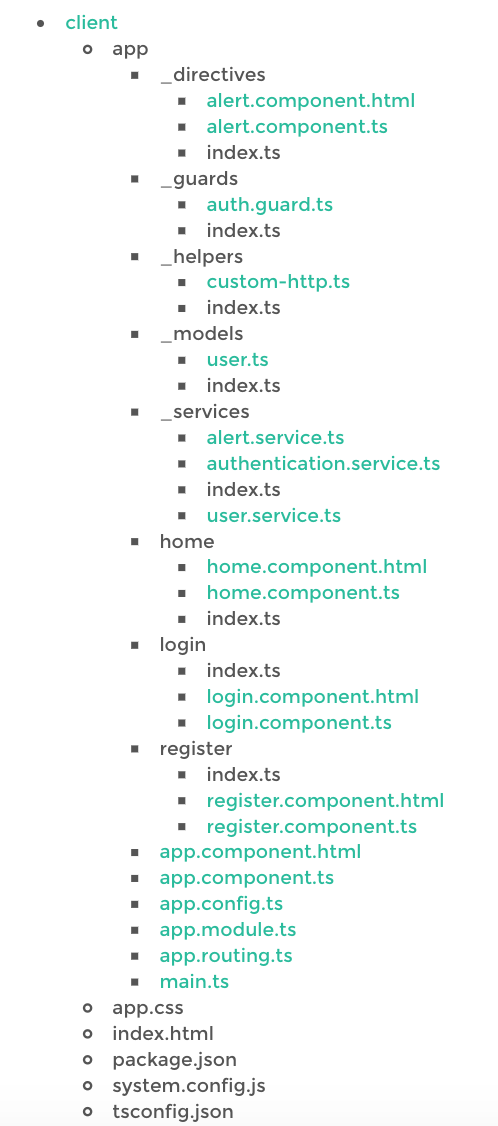
\includegraphics[width=40mm]{img/aplicacion/cliente.png}
    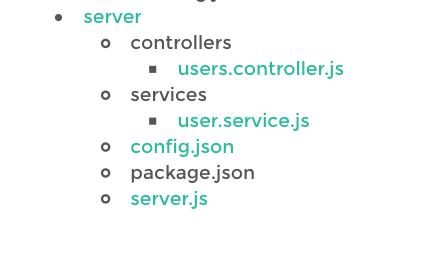
\includegraphics[width=40mm]{img/aplicacion/server.png}
    \caption{Estructura de un proyecto con la pila MEAN}
    \label{img:EstructuraMean}
\end{figure}
\section{Lado cliente de la aplicación web}

De los 8 bloques principales de una app en Angular, vamos a ir identificando uno a uno y que uso se le da en nuestra aplicación.

\subsection{Modulos: } Como las aplicaciones en Angular son modulares y un módulo es el conjunto de código dedicado a cumplir un único objetivo, los módulos utilizados en nuestra aplicación son:
\begin{itemize}
\item \textbf{NgModule from '@angular/core'} Es el módulo principal, el cual recibe un objeto que define el módulo. Los metadatos más importantes de un NgModule son:

\begin{enumerate}
\item{Declarations: } Las vistas que pertenecen a tu módulo. Hay 3 tipos de clases de tipo vista: componentes, directivas y pipes.
\item{Exports: } Conjunto de declaraciones que deben ser accesibles para plantillas de componentes de otros módulos.

\item{Imports: } Otros NgModules, cuyas clases exportadas son requeridas por templates de componentes de este módulo.

\item{Providers: } Los servicios que necesita este módulo y que estarán disponibles para toda la aplicación.

\item{Bootstrap: }: Define la vista raíz. Utilizado sólo por el root module.
\end{enumerate}

\item \textbf{RouterModule from '@angular/router'} es uno de los módulos más importantes de Angular, se encuentra dentro de la librería @angular/route, gracias a él cada vez que cambiemos de direccion URL cambiaremos de página sin necesidad de tener que interactuar con el servidor.

\item \textbf{ HttpModule, Http, RequestOptions from '@angular/http'} Otro módulo imprescindible en una aplicación Angular, se encuentra dentro de la librería @angular/http. Gracias a este módulo podemos hacer cualquier petición AJAX sin apenas tener que escribir código.

\item \textbf{ FormsModule from '@angular/forms'} Módulo encargado de añadir formularios personalizados.

\item \textbf{FileUploadModule from 'ng2-file-upload'} Es el módulo que nos permite subir imágenes y enviarlas a nuestro servidor, para luego poder almacenarlas de forma ordenada en nuestra base de datos.

\item \textbf{AgmCoreModule from 'angular2-google-maps/core} Gracias a este módulo, podemos utilizar la API de google maps en nuestra aplicación.

\item \textbf{ BrowserModule from '@angular/platform-browser'} Este módulo es necesario en cualquier app que se renderice en el navegador.


\item \textbf{ AuthGuard from './common/auth.guard'} Gracias a este modulo, podemos conservar las credenciales de un usuario durante un tiempo determinado en el navegador.

\item \textbf{ ProvideAuth, AuthHttp, AuthConfig from 'angular2-jwt'} Este módulo proporciona seguridad a nuestra aplicación, generando un \textit{token} encriptado para cada usuario que se registre en nuestra aplicación.

\item \textbf{AppComponent, Intro, LoginAlumno, LoginProfesor , HomeAlumno, HomeProfesor, SignupAlumno, SignupProfesor, ProfesorDetail } Estos son los módulos propios se han desarrollado para la aplicación de este TFG.
\end{itemize}
\subsection{Componentes: }

Los componentes son como etiquetas nuevas que podemos inventarnos para realizar las funciones que sean necesarias para nuestra aplicación de gestión de clases particulares.

Se compone de 1 componente principal y 8 componentes que derivan de él. AppComponent es el componente principal y tiene la siguiente apariencia:

\begin{lstlisting}[caption=AppsComponent]
import { Component } from '@angular/core';

@Component({
  selector: 'app-root',
  templateUrl: './app.component.html',
  styleUrls: ['./app.component.css']
})
export class AppComponent {
  title = 'ClassCity';
}
\end{lstlisting}

El selector app-root o el nombre de la etiqueta que se usará cuando se desee representar. Con la propiedad templateUrl asociamos un archivo .html que se usará como vista del componente. Por último se define su estilo mediante la propiedad StyleUrls, indicando a un array de todas las hojas de estilos que deseamos.

\subsubsection{Componentes secundarios }

\begin{itemize}
\item \textbf{Intro} Este componente corresponde con la página introductoria a la aplicación donde podemos elegir entre qué perfil de usuario queremos adoptar: Profesor o Alumno. Como podemos ver en la figura \ref{img:introclasscity}.

\item \textbf{LoginAlumno, LoginProfesor} Componentes encargados de realizar la función de login del alumno o del profesor como podemos ver en las figuras \ref{img:loginalumnoclasscity} \ref{img:loginprofesorclasscity}. Hemos desarrollado una función que se encarga de realizar una petición POST al servidor. Si la respuesta es aceptada, el alumno accedera a la aplicación y se almacenarán las credenciales en el \textit{localstorage} del navegador con un tiempo de caducidad de 1 hora. Mientras que si la petición es rechazada, el servidor nos enviará un mensaje avisando de que \textit{The username or password don't match}.

\item \textbf{SignupAlumno, SignupProfesor} Estos componentes se van a encargar de registrar a profesores y alumnos en nuestra base de datos. Para ellos hemos desarrollado una función en cada componente que simplemente se encarga de enviar al servidor una petición POST con un cuerpo donde se encuentran los datos personales del profesor o el alumno. Figura \ref{img:signupalumnoclasscity} \ref{img:signuprofesorclasscity}

\item \textbf{HomeAlumno, HomeProfesor} Cuando un profesor o un alumno es aceptado dentro de nuestra base de datos y consigue entrar en la aplicación, puede realizar diferentes funciones dependiendo de si entro como alumno o como profesor. figuras \ref{img:homealumnoclasscity} \ref{img:homeprofesorclasscity}.

\begin{enumerate}
\item \textbf{Alumno }  Un alumno puede realizar la búsqueda del profesor que más le interese por diferentes parámetros:
\begin{itemize}
    \item{El curso en el que está el alumno}
    \item{La asignatura que quiere cursar}
    \item{La distancia a la que se encuentre el profesor}
\end{itemize}

\item \textbf{Profesor } La página del profesor consiste en un chat realizado con \textit{websockets}, donde podrá entablar conversación con cualquier alumno que este interesado en él. Aparte puede personalizar su perfil, cambiando la foto que tiene como avatar.
\end{enumerate}

\item \textbf{ProfesorDetail} Cuando un alumno encuentra a su profesor particular ideal desde la página del alumno y hace click sobre el profesor interesado, el componente ProfesorDetail se lanza y consiste en una ficha técnica del profesor particular, así como un chat donde el alumno podrá comunicarse con el profesor para poder quedar y acordar el precio de la clase tal y como podemos ver en la figura \ref{img:detailprofesorclasscity}

\end{itemize}

\subsection{Plantilla }

Las plantillas se utilizan para dar forma a las aplicaciones. Es la parte más visual de una aplicación web y es la propia magia de Angular la que se encarga de renderizar estas plantillas, haciendo aplicaciones mucho más personalizadas para el usuario. A continuación vamos a ir analizando una a una las diferentes plantillas que forman la aplicación de gestión de clases particulares:

\textbf {intro.html} Cuando accedemos a la URL \footnote{\url{https://www.classcity.es}} de la aplicación, la primera plantilla que se nos presenta es Intro.html. Según podemos ver en la imagen  \ref{img:introclasscity}, consiste en una página introductoria donde podemos elegir si somos alumnos o porfesores.

\begin{figure}[!h]
    \centering
    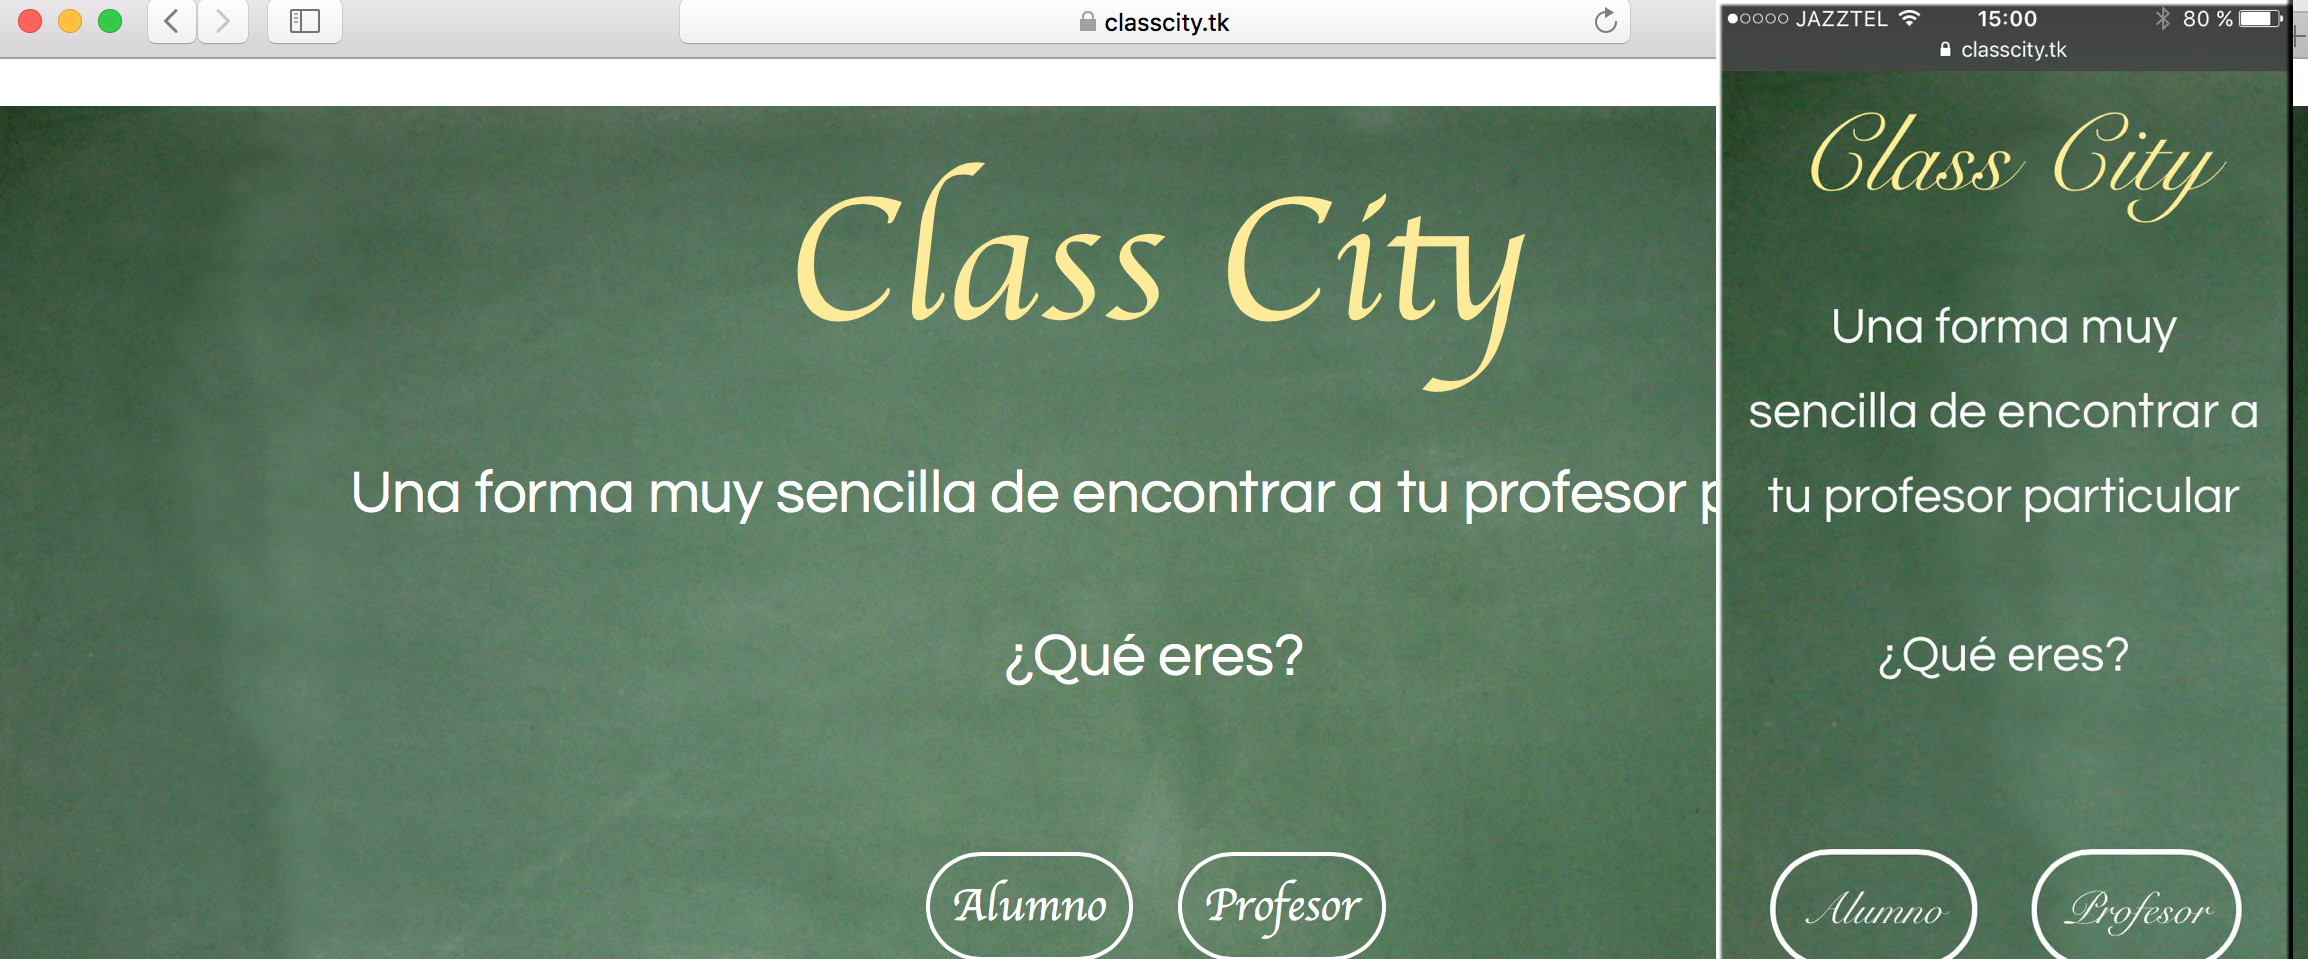
\includegraphics[width=140mm]{img/templates/intro.png}
    \caption{Página Intro ClassCity}
    \label{img:introclasscity}
\end{figure}


\textbf{loginalumno.html} Al seleccionar dentro de Intro.html en Alumno, accedemos a la siguiente plantilla donde podemos visualizar un formulario con sus campos \textit{username} y \textit{password}. Además de resaltar la caracteristica resposive de la aplicación, demostrando que es totalmente adaptable para dispositivos moviles como para ordenadores.

\begin{figure}[!h]
    \centering
    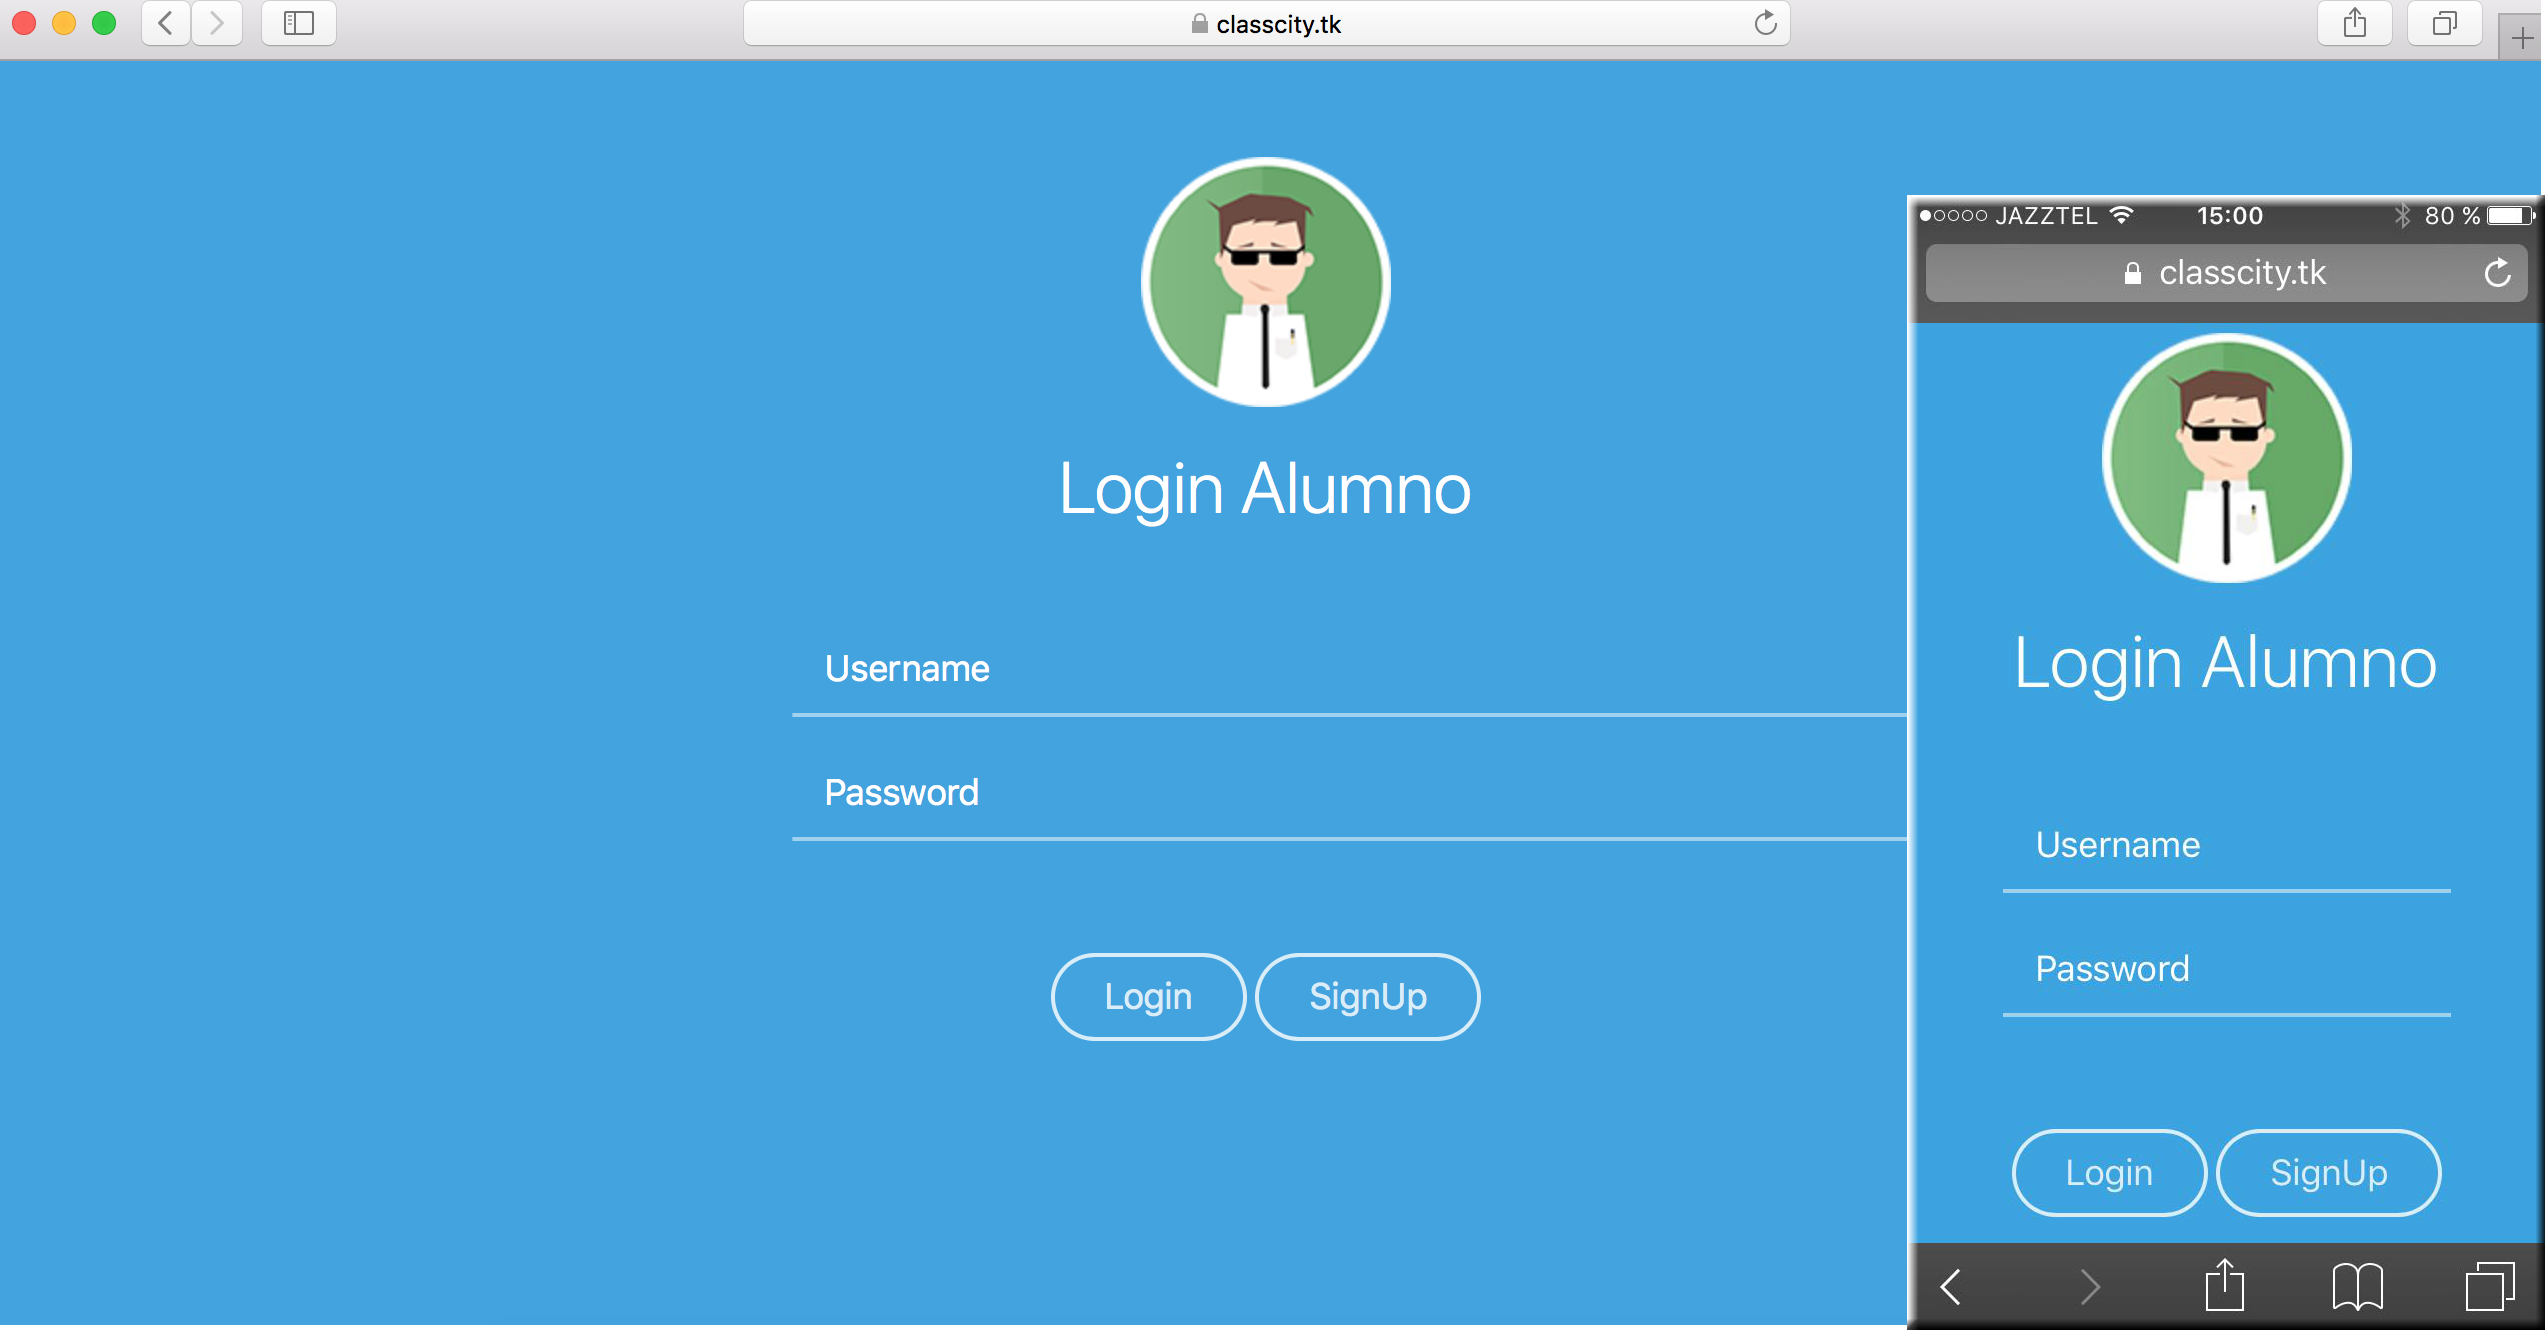
\includegraphics[width=140mm]{img/templates/loginalumno.png}
    \caption{Página Login Alumnos}
    \label{img:loginalumnoclasscity}
\end{figure}


\textbf{loginprofesor.html} Si en vez de seleccionar Alumno hubiésemos seleccionado Profesor en la página introducctoria, hubiesemos entrado en otro formulario donde los profesores ya registrados pueden acceder a la aplicación.Al igual que la plantilla de \textit{loginalumno.html} es totalmente resposive. Para poder controlar que la plantilla sea resposinve hemos utilizado diferentes ficheros css \textit{(movil.css y ordenador.css)} por cada plantilla en todas las plantillas de la aplicación.
\begin{figure}[!h]
    \centering
    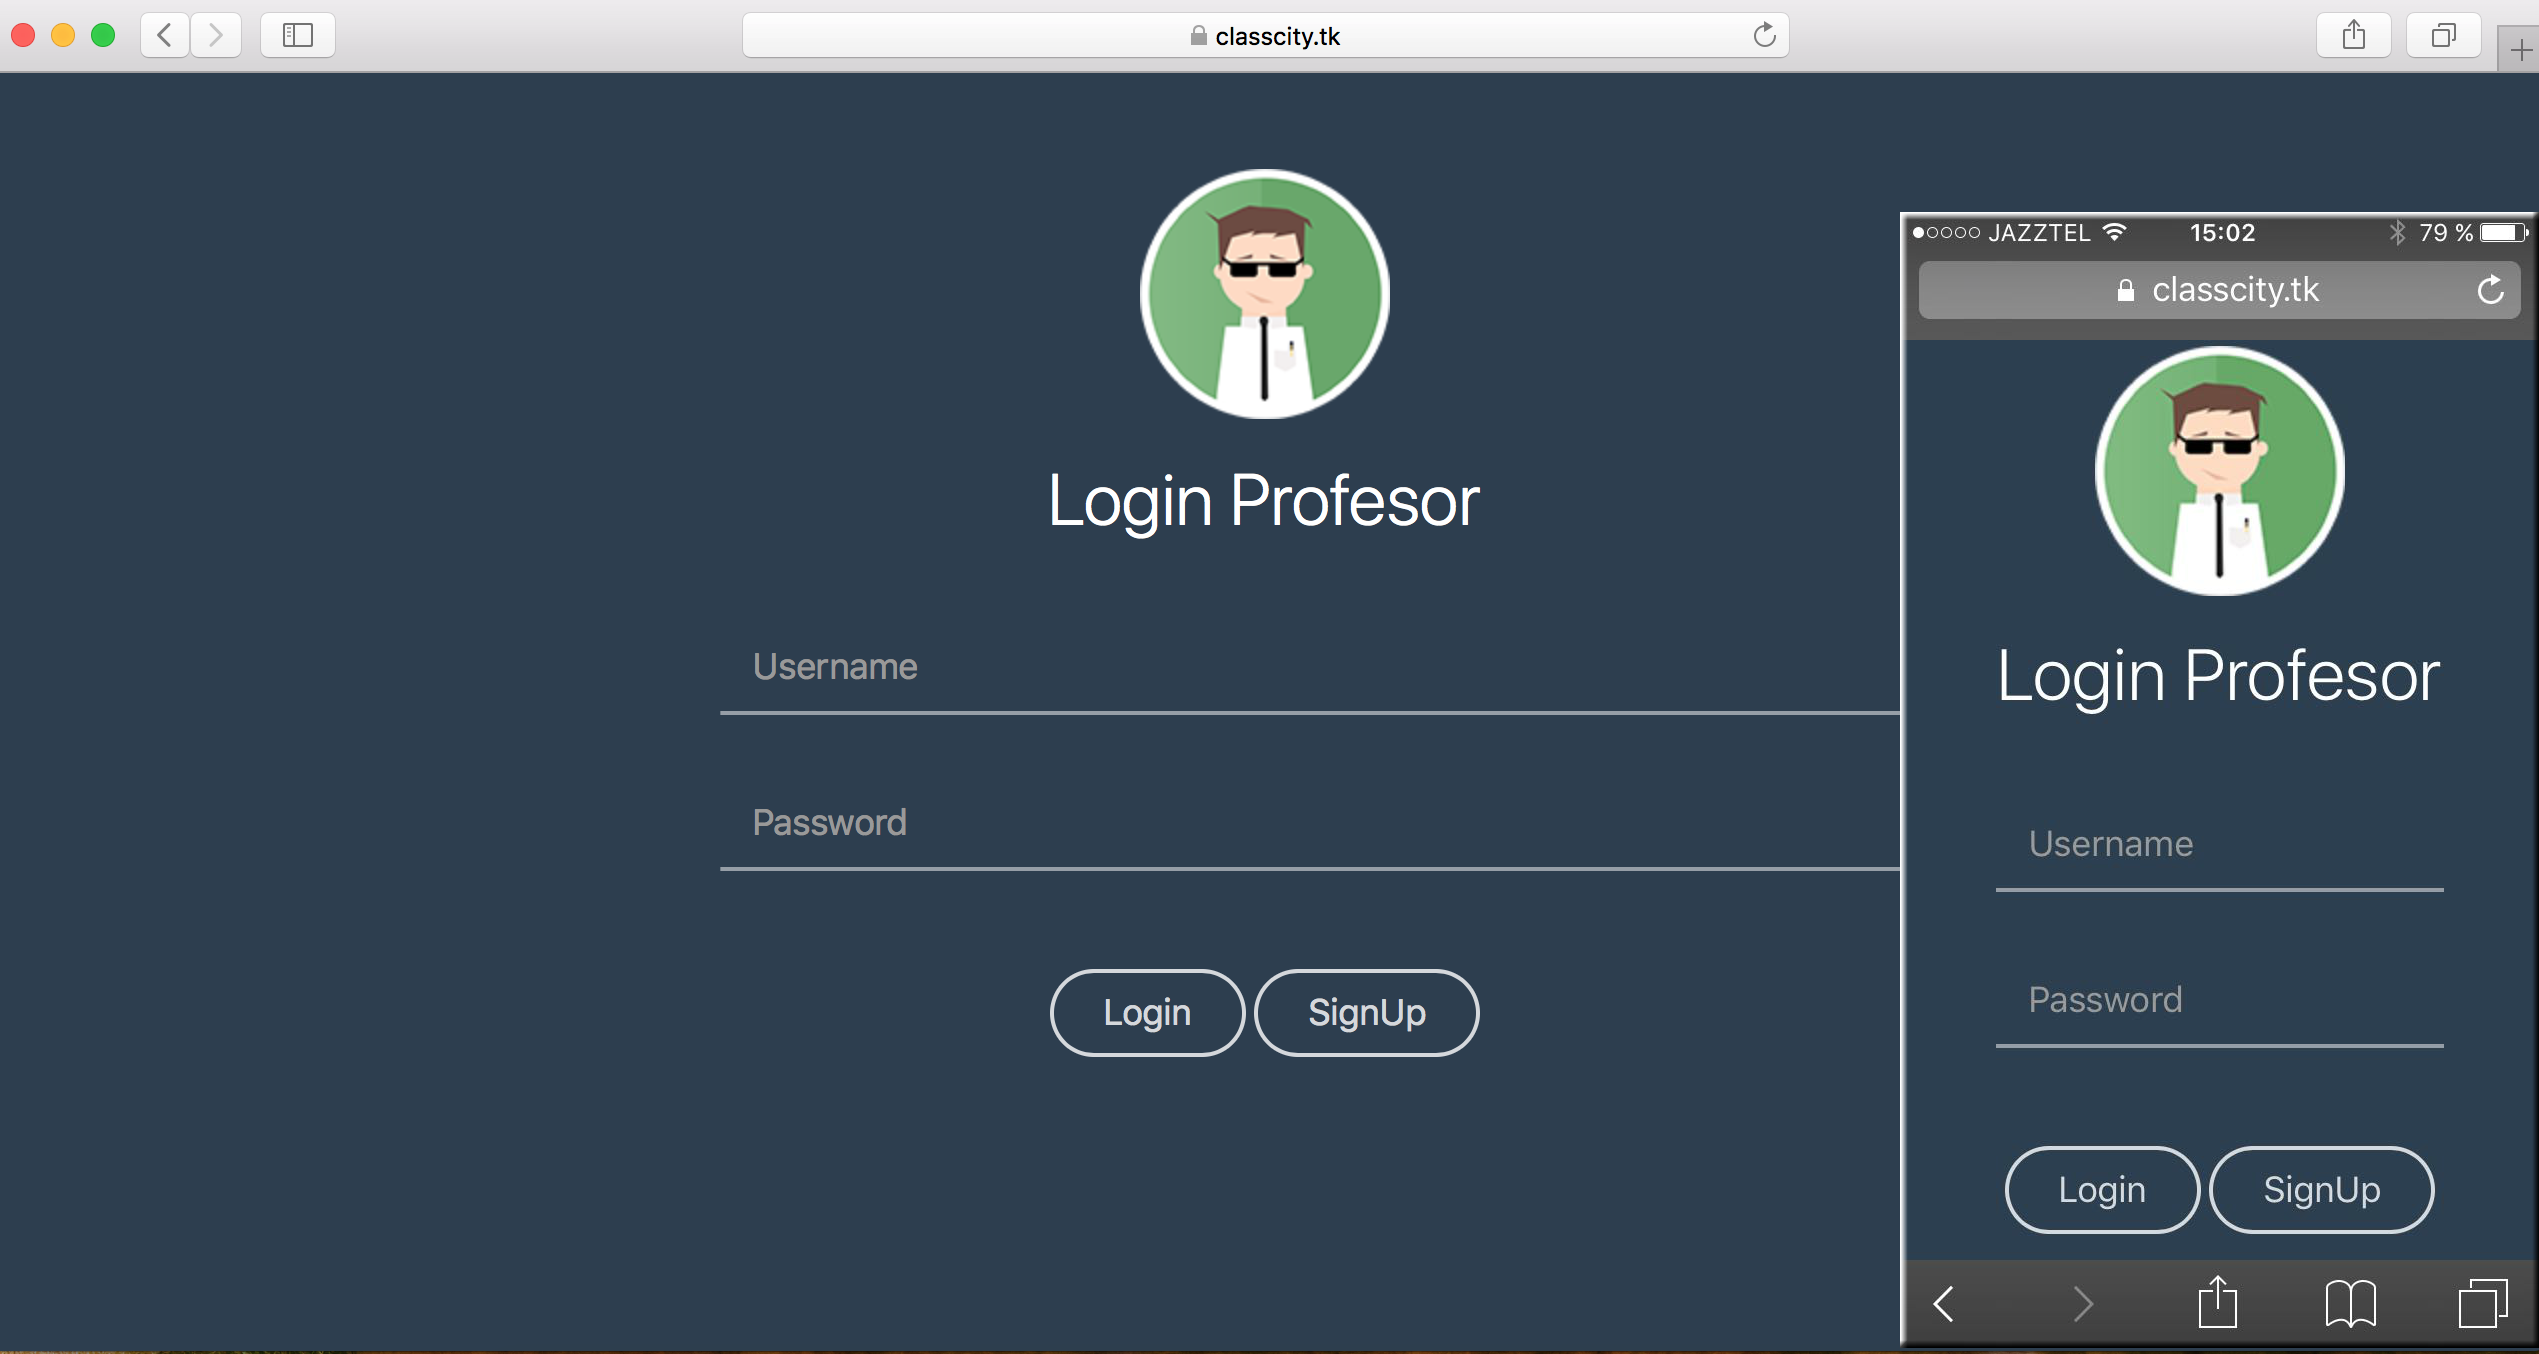
\includegraphics[width=140mm]{img/templates/loginprofesor.png}
    \caption{Página Login Profesor}
    \label{img:loginprofesorclasscity}
\end{figure}

\textbf{registeralumno.html} Si un alumno quiere registrase simplemente debe entrar en SignUp, donde tendrá un formulario para poder completar todos los campos necesarios. Los datos que solicitamos para el alumno son los siguientes: Email, Password, Nombre, Apellidos y Fecha de Nacimiento. Todos estos datos serán enviados a nuestro servidor donde almacenaremos la información.
\begin{figure}[!h]
    \centering
    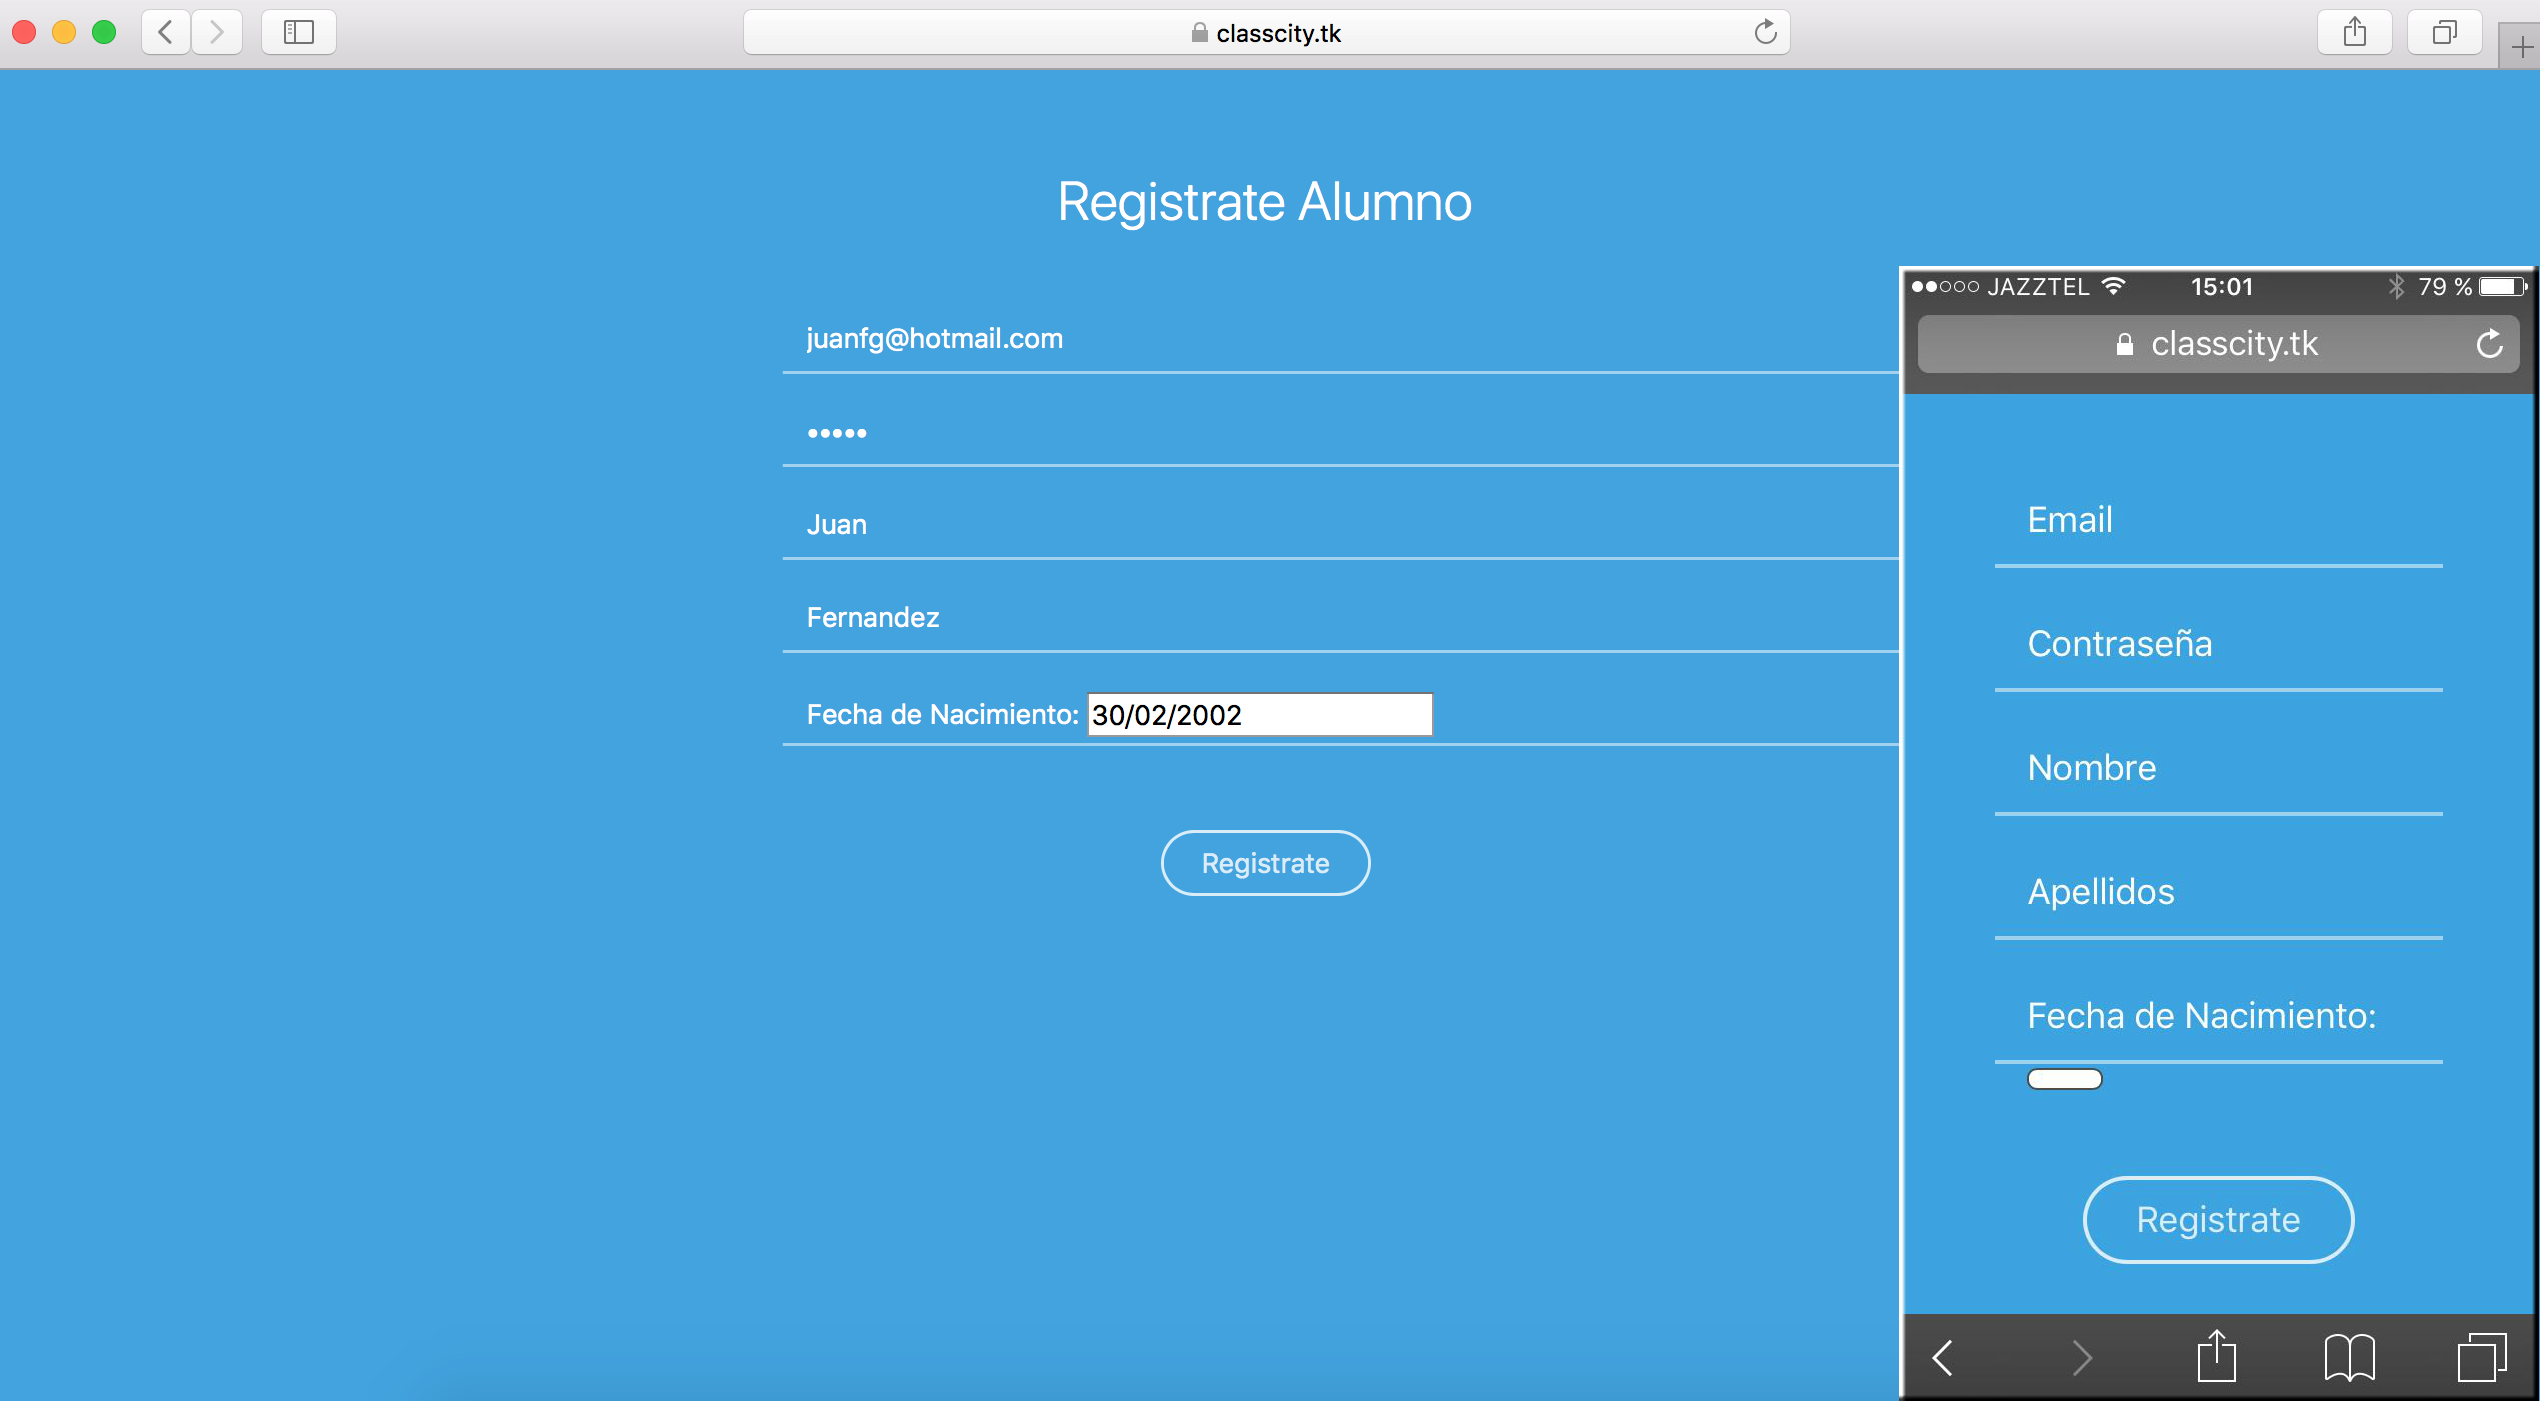
\includegraphics[width=140mm]{img/templates/registeralumno.png}
    \caption{Página Registrar Alumno}
      \label{img:signupalumnoclasscity}
\end{figure}

\textbf{registerprofesor.html} Si es el profesor quien quiere registrarse en nuestra aplicación, entrará en SignUP de profesores e introducirá los datos necesarios. Los datos que solicitamos al profesor son: Ubicación, Nombre, Apellidos, Password, Email, Fecha de Nacimiento, Curso y Asignatura.
\begin{figure}[!h]
    \centering
    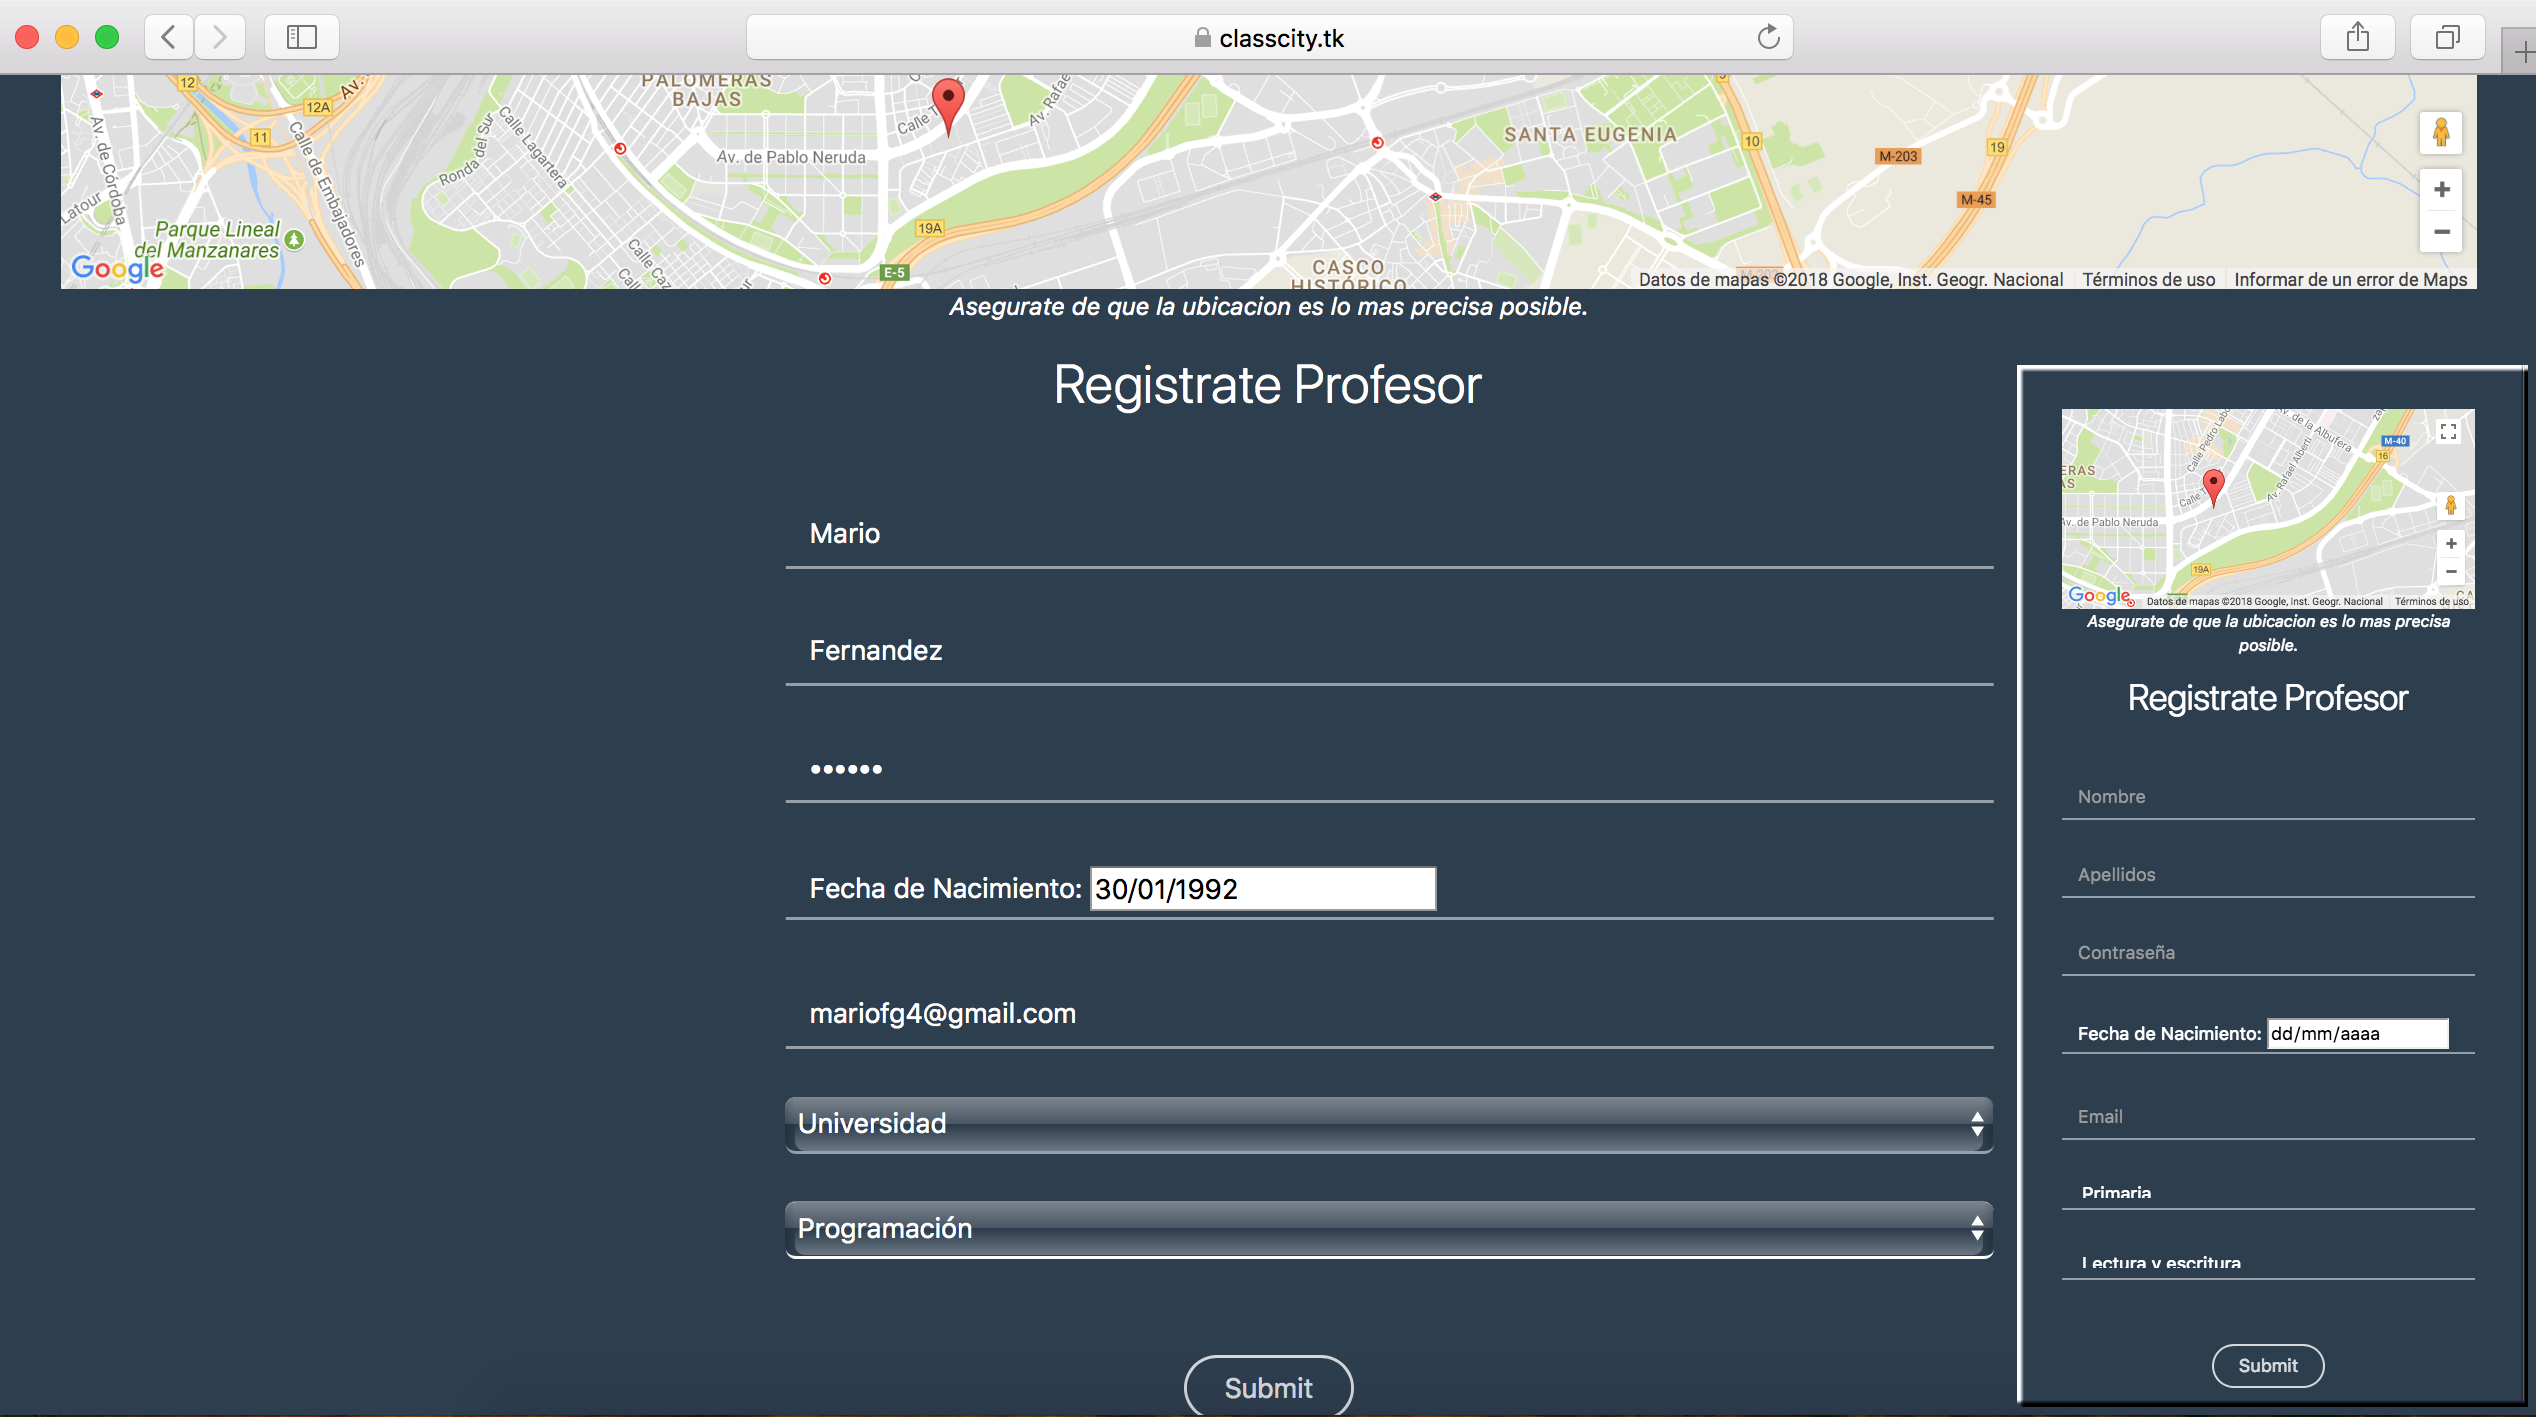
\includegraphics[width=140mm]{img/templates/registerprofesor.png}
    \caption{Página Registrar Profesor}
    \label{img:signuprofesorclasscity}
\end{figure}

\textbf{homealumno.html} Una vez que el alumno ya ha sido registrado en nuestra base de datos, la interfaz con la que se encontrará el es la que podemos ver en la figura \ref{img:homealumnoclasscity}.
Podemos apreciar una entrada en el mapa para introducir la ubicación donde queremos buscar. También podemos diferenciar los filtros de búsqueda que tenemos para buscar a nuestro profesor. Por último, cuando el alumno busca con los parámetros que desee, les aparecerán pintados en el mapa tantos profesores como haya en nuestra aplicación con esas especificaciones.
\begin{figure}[!h]
    \centering
    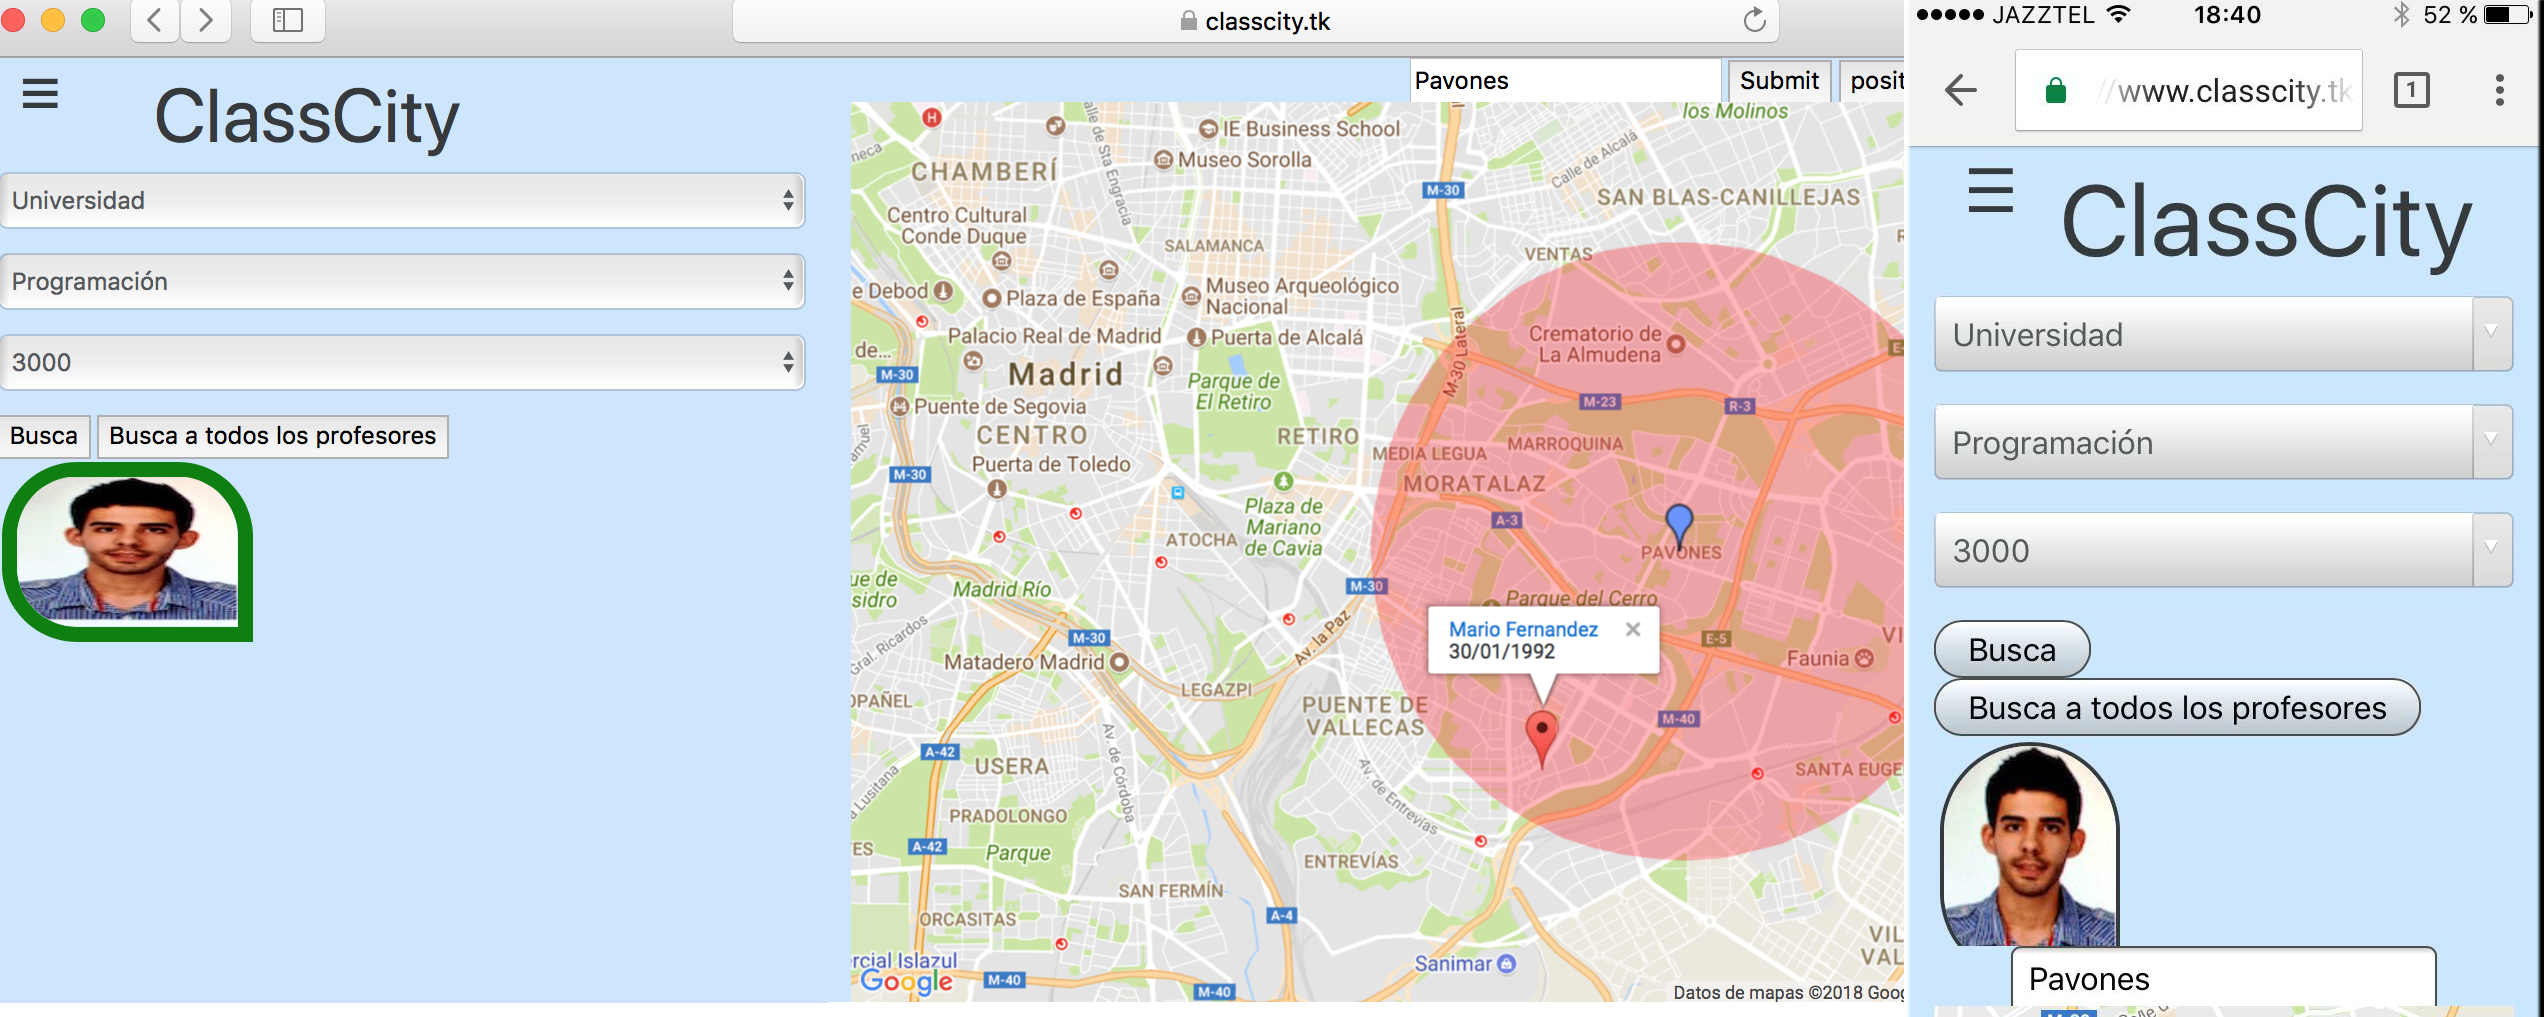
\includegraphics[width=160mm]{img/templates/homealumno.png}
    \caption{Página Home Alumno}
    \label{img:homealumnoclasscity}
\end{figure}

\textbf{detail.html} Cuando el alumno encuentra algún profesor de su interés puede hacer click sobre la imagen del profesor y así entrar en más detalle, viendo su ficha técnica y pudiendo entablar una conversación a partir del chat. La ficha técnica muestra los siguientes datos del profesor: Nombre, Apellidos, Asignatura y Curso.
\begin{figure}[!h]
    \centering
    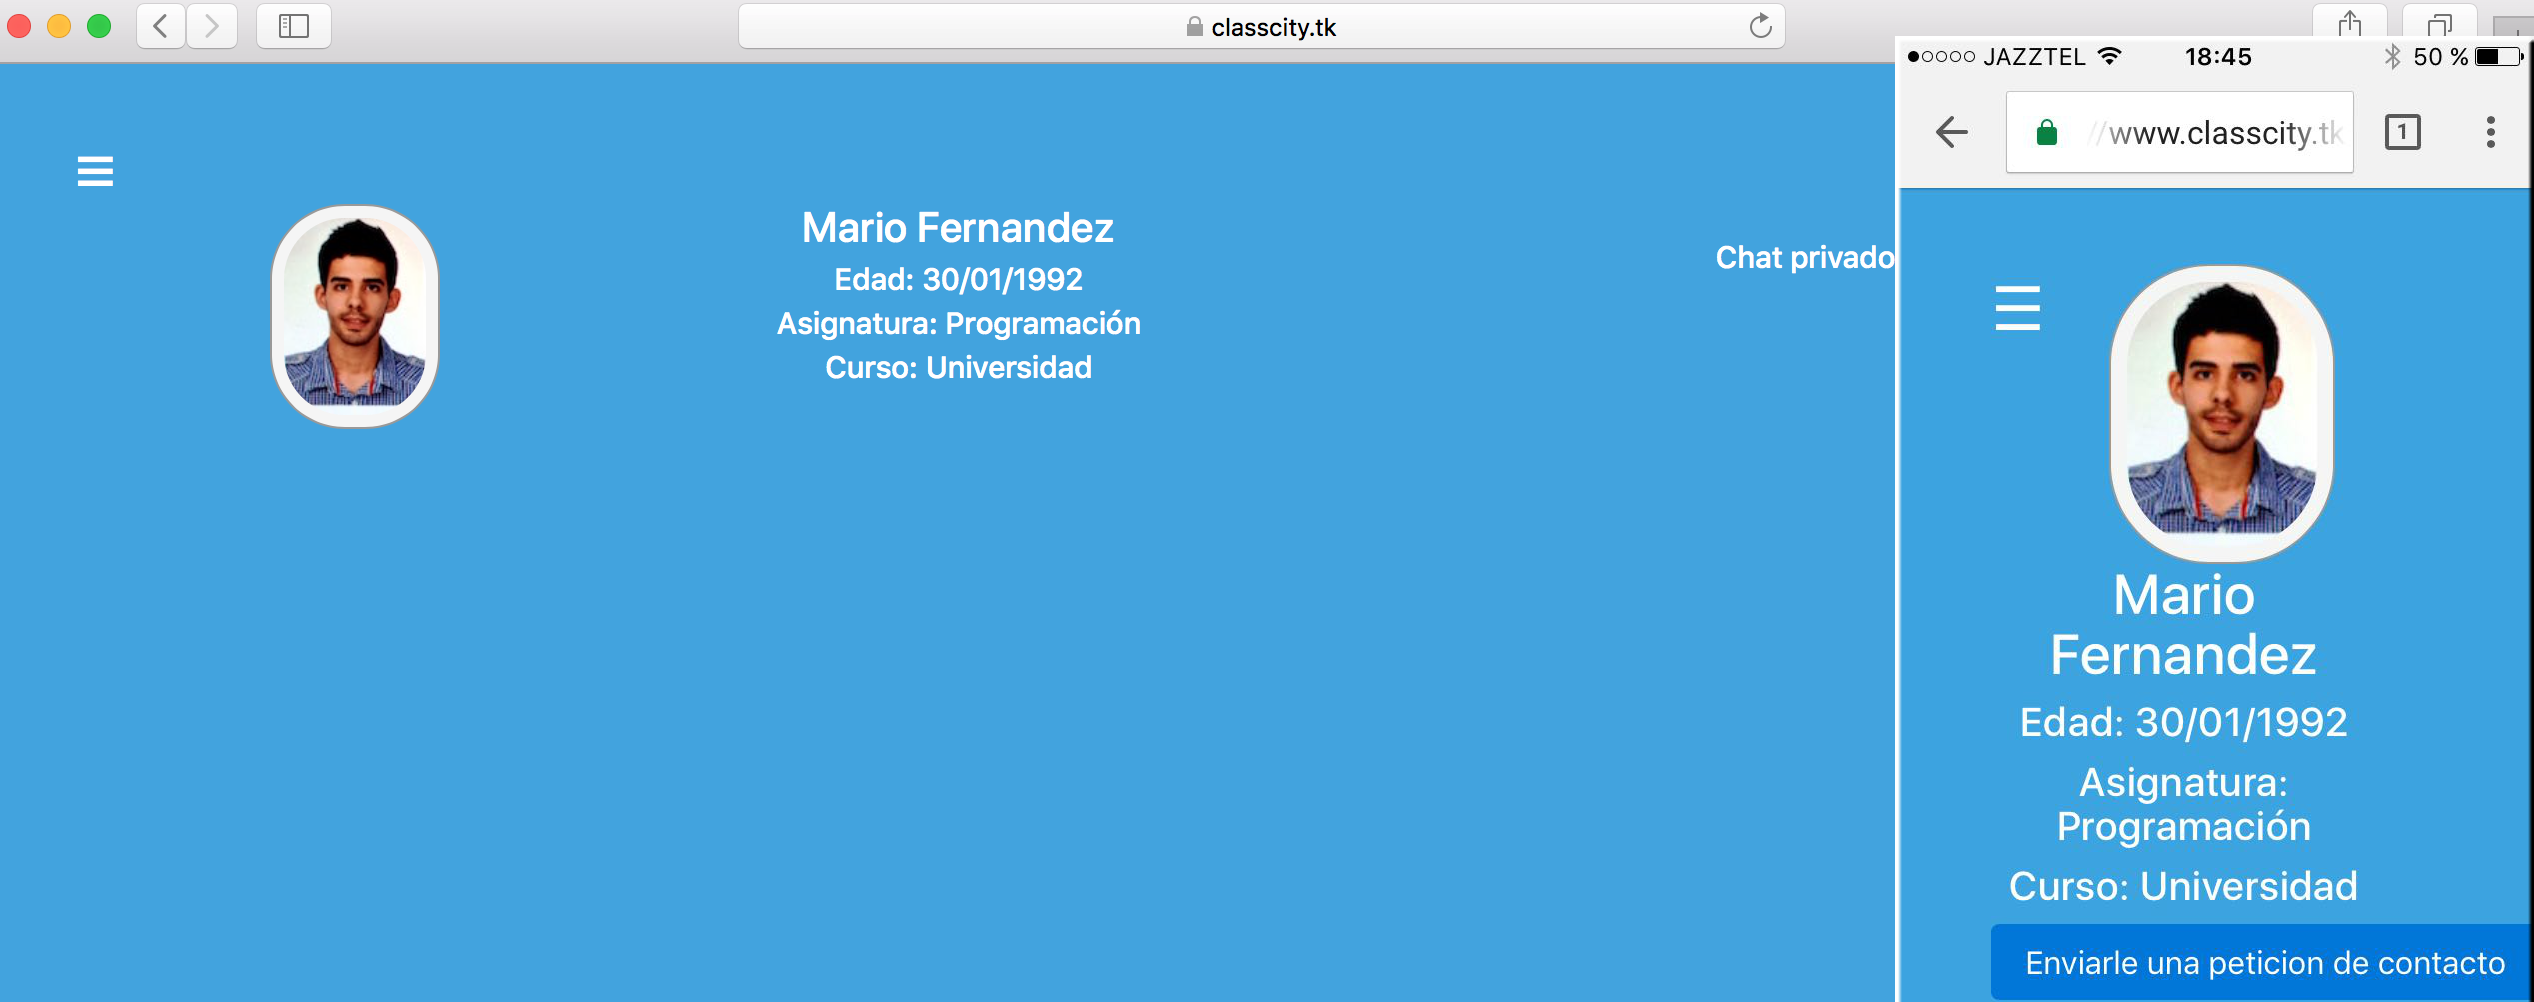
\includegraphics[width=160mm]{img/templates/detailprof.png}
    \caption{Página Detalle del Profesor}
    \label{img:detailprofesorclasscity}
\end{figure}

\textbf{homeprofesor.html} Cuando el profesor ya ha sido registrado en nuestra aplicación, el home del profesor es habilitado y en él puede hablar por un chat privado con todos los alumnos que le escriban por su canal, además de poder editar la foto de su perfil.
\begin{figure}[!h]
    \centering
    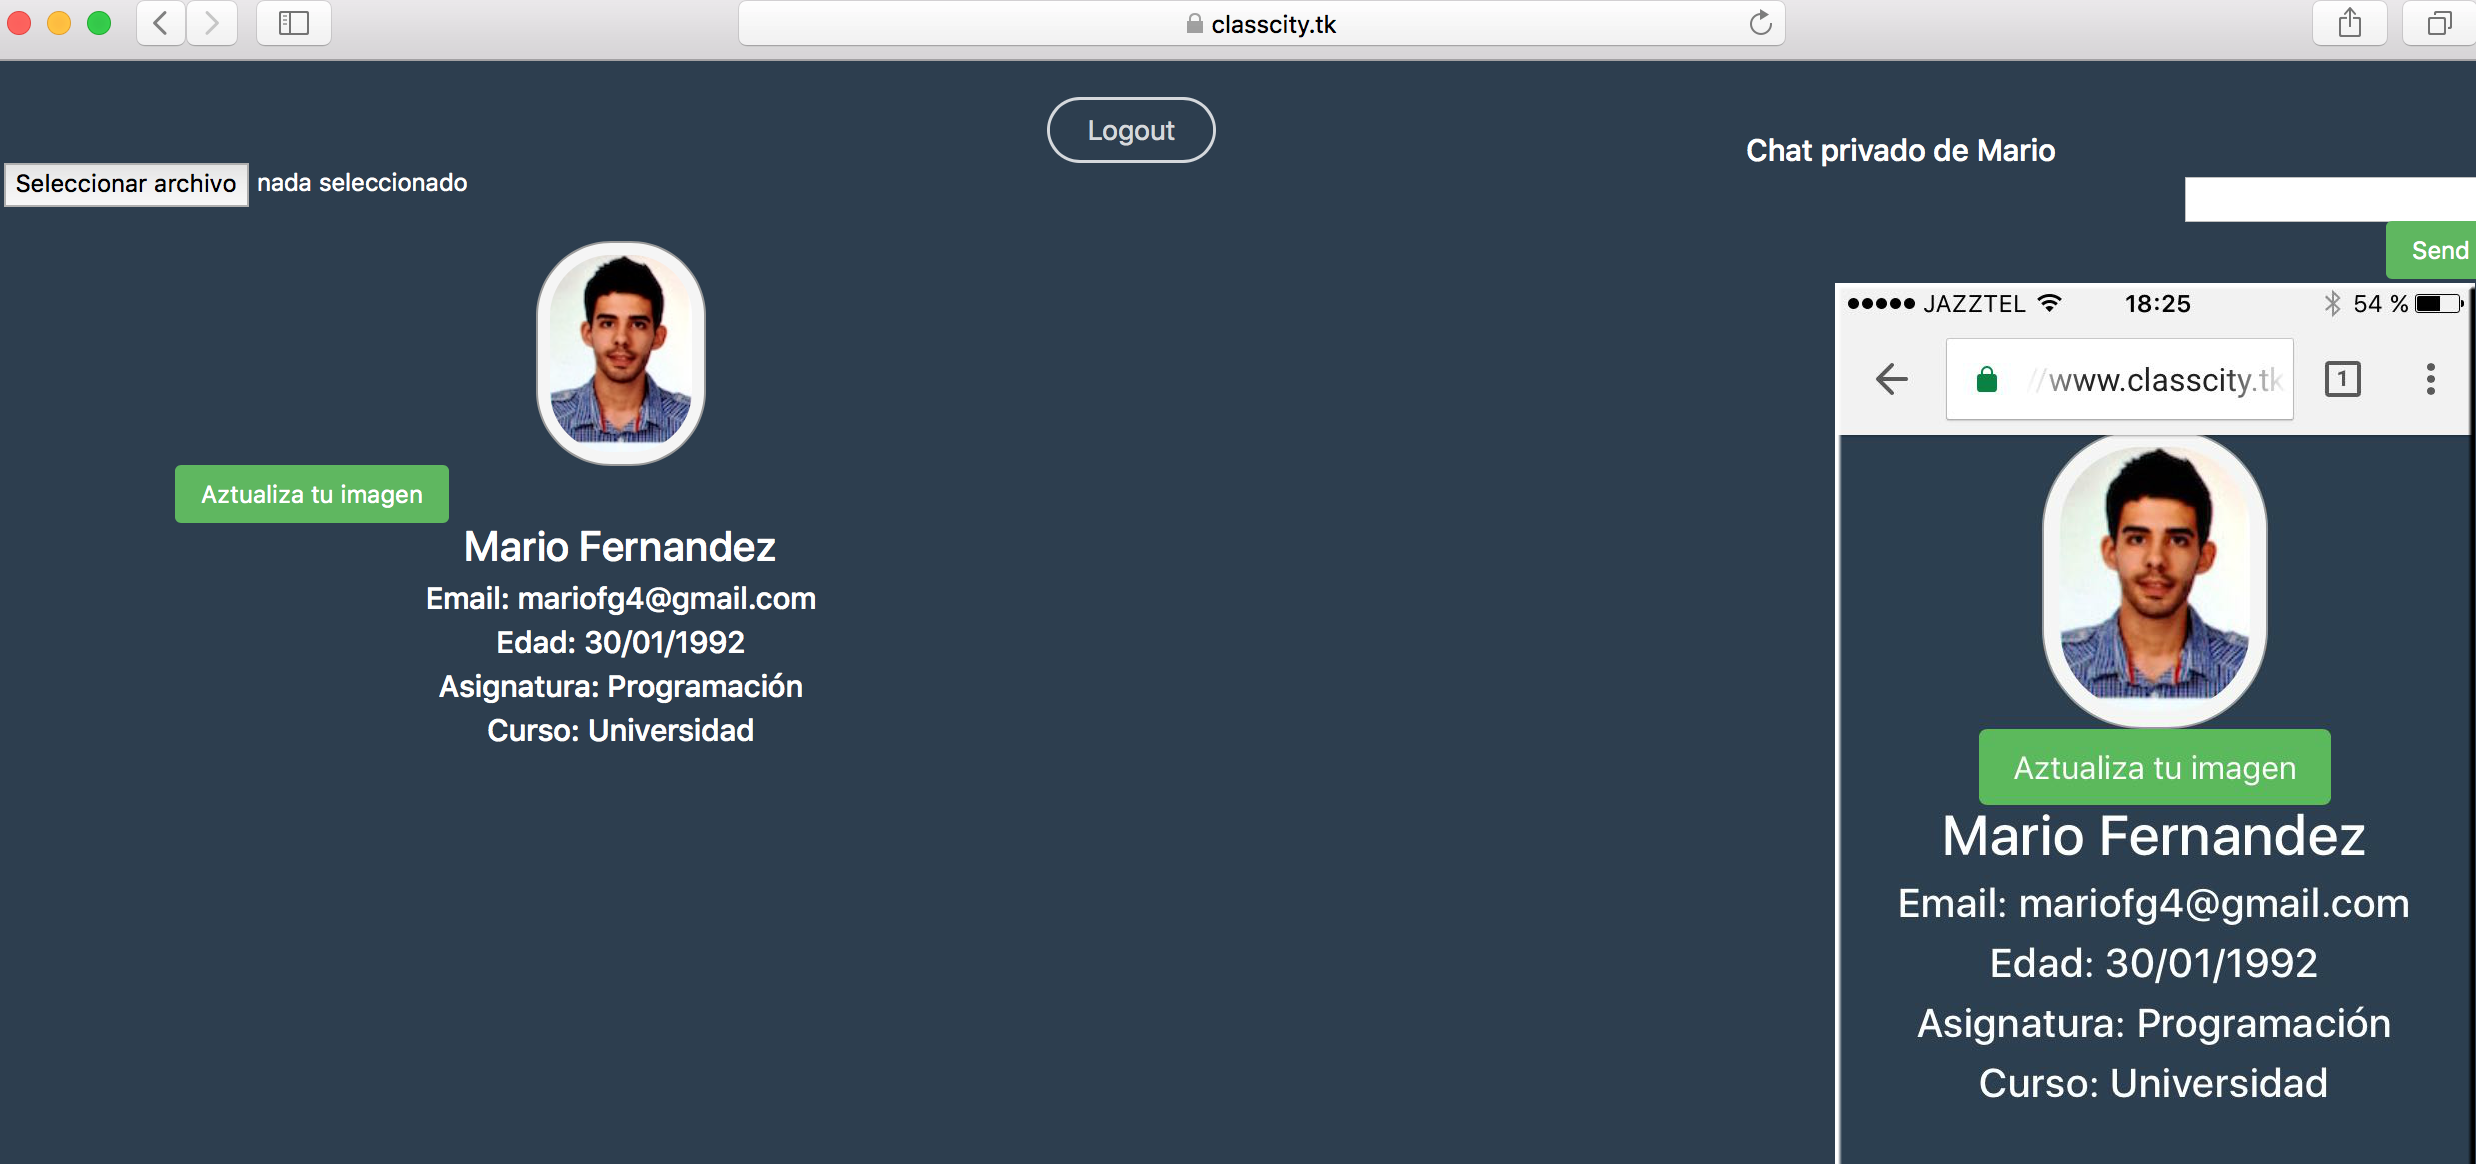
\includegraphics[width=160mm]{img/templates/homeprof.png}
    \caption{Página Home Profesor}
    \label{img:homeprofesorclasscity}
\end{figure}

\subsection{Data Binding} El Data Binding nos abstrae de la lógica \textit{pull/push} asociada a insertar y actualizar valores en el HTML y convertir las respuestas de usuario(inputs, clicks, etc) en acciones concretas.

Como se ha comentado en el capítulo anterior Angular tiene 4 formas de Data Binding, todas ellas se han utilizado en nuestra aplicación para realizar las siguientes funciones:

\textbf{Interpolación(Hacia el DOM)} Angular evaluá todas las variables e introduce su resultado en el DOM. En el siguiente ejemplo estamos insertando en el árbol DOM, todos los datos del usuario, consiguiendo una apariencia de la página mucho más personalizada.

\begin{lstlisting}
<code>{{decodedJwt.Email}}</code></pre>
<code>{{decodedJwt.id.nombre}}</code></pre>
<code>{{decodedJwt.id.apellidos}}</code></pre>
<code>{{decodedJwt.id.edad}}</code></pre>
\end{lstlisting}

\textbf{Property binding: (Hacia el DOM))} Este tipo de Data Binding, permite pasar los objetos que queramos de nuestro componente padre ('home') a la propiedad (Latitud, Longitud, radius, fillColor) del componente hijo, en este caso sebm-google-map-circle. Para ello el componente hijo tiene que tener predefinidas ciertas entradas en su directiva.

\begin{lstlisting}
<sebm-google-map-circle
    [latitude]="query.Loc.lat"
    [longitude]="query.Loc.lng"
    [radius]="query.Radio"
    [fillColor]="'red'">
</sebm-google-map-circle>
\end{lstlisting}

\textbf{Event binding: (Desde el DOM)}
Si queremos invocar a una función cuando se lance un evento, como por ejemplo cuando queremos hacer click en el botón de LogOut. En el momento que hacemos click sobre el boton de logout, la función logout es invocada y salimos de la sesión.

\begin{lstlisting}
<button type="Submit" (click)="logout()">Logout</button>
\end{lstlisting}

\textbf{Two-way binding: (Desde/Hacia el DOM)}

Cuando queremos combinar el \textit{Event Binding y el Property Binding} tenemos el binding bi-direccional, como podemos ver en el siguiente ejemplo.

\begin{lstlisting}
<input [(ngModel)]="address">
\end{lstlisting}

En este caso queremos que el valor de 'address' se actualice en el componente y que a su vez se introduzca dentro de la entrada como en el caso de \textit{property binding}.

\subsection{Directiva: }Las directivas son como los componentes, pero sin una plantilla asociada. En nuestro caso hemos utilizado directivas para realizar varias funciones, por ejemplo:

\textbf{FileSelectDirective, FileDropDirective, FileUploader} Estas tres directivas proceden del módulo "FileUploadModule", y sirven para poder subir una imagen desde el escritorio local del usuario al navegador, para luego enviar la imagen al servidor.

\begin{lstlisting}
<input type="file" ng2FileSelect [uploader]="uploader" />
\end{lstlisting}
\textbf{sebm-google-map, sebm-google-map-marker} Estas son otras de las directivas procedentes del módulo 'agmCoreModule', el cual nos proporciona toda la interfaz de programación de GoogleMaps. Gracias a estas directivas podemos jugar con el API de google en nuestra aplicación angular.

\begin{lstlisting}
<sebm-google-map *ngIf="query.Loc"
    [latitude]="query.Loc.lat"
    [longitude]="query.Loc.lng"
    [scrollwheel]="false" [zoom] = "13">
    <sebm-google-map-marker
        [latitude]="query.Loc.lat"
        [longitude]="query.Loc.lng"
        [iconUrl] = "iconUrl">
    </sebm-google-map-marker>
</sebm-google-map>
\end{lstlisting}

También hemos usado otros dos tipos de directivas que hemos usado en nuestra aplicación.

\textbf{Directivas Estructurales: *ngFor} repite su elemento en el DOM una vez por cada item que hay en el iterador que se le pasa, siguiendo una sintaxis de ES6.

\textbf{Directivas Atributo: ngModel} Implementa un mecanismo de binding bi-direccional. En este ejemplo el elemento HTML $<$select$>$, asigna la propiedad value a mostrar y además responde a eventos de modificación.
\begin{lstlisting}
<div class="form-group">
    <select class="form-control" [(ngModel)]="query.Curso" name="curso">
        <option *ngFor="let p of curso" [value]="p">{{p}}</option>
    </select>
</div>
\end{lstlisting}

\subsection{Servicio } Los servicios se definen a través de simples clases y son imprescindibles en Angular, ya que toda función o valor es encapsulada dentro de un servicio.

\textbf{AlumnoService} Este servicio se encarga de convertir una dirección física a una coordenada (latitud, longitud) para poder representarlo en el mapa.

Si observamos detenidamente el código, lo primero que hacemos en la función 'getLatLan(address: string)', es una petición al API de Google maps con una dirección y esperamos a que nos responda. La respuesta puede ser satisfactoria o no. En caso de que sea OK las variables lat y lng serán actualizadas con los valores devueltos por Google maps. Si por el contrario no hubiésemos recibido respuesta, un mensaje de error será mostrado por pantalla.
\begin{lstlisting}
export class AlumnoService {
  getLatLan(address: string) {
    let geocoder = new google.maps.Geocoder();
    return Observable.create(observer => {
      geocoder.geocode( { 'address': address}, function(results, status) {
        if (status === google.maps.GeocoderStatus.OK) {
          let obj: Object = {lat: results[0].geometry.location.lat(),
            lng: results[0].geometry.location.lng() };
            observer.next(obj);
            observer.complete();
        } else {
            console.log('Error - ', results, ' & Status - ', status);
            observer.next({});
            observer.complete();
        }
      });
    });
  }
}
\end{lstlisting}

\section{Lado servidor de la aplicación}

Nuestro lado servidor se compone de dos tecnologías muy importantes e innovadoras en el mercado de las aplicaciones web como son: Express, que como ya hemos comentado antes es un framework de desarrollo de aplicaciones web para Node.js y MongoDB que consiste en una base de datos NoSQL, el cual utiliza la librería \textit{mongoose} para poder conectar node.js con la base de datos en MongoDB.
Como ya he comentado en el capítulo anterior, Node es es un sistema innovador, puesto que es la plataforma encargada del funcionamiento del servidor, y funciona totalmente con JavaScript. Gracias a Node, simplemente con una linea en la terminal seremos capaces de generar procesos que escuchen en el puerto que queramos.
Una vez tengamos \textit{Node(v10.0.0) y NPM(5.6.0)} instalados, procedemos a instalar las dependencias tanto del servidor como del cliente y posteriormente arrancar la aplicación.

\begin{itemize}

\item textbf{Instalar dependencias(Cliente y Servidor)}
\begin{lstlisting}
    sudo npm install
\end{lstlisting}
\item  \textbf{Correr nuestro servidor}
\begin{lstlisting}
    sudo node server.js
\end{lstlisting}
\item  \textbf{Arrancar el cliente: }
\begin{lstlisting}
    sudo npm start
\end{lstlisting}
\end{itemize}

\subsection{Server.js}

Las funciones contenidas en nuestra server.js son:

\begin{enumerate}
    \item \textbf{Open mongo} Llamamos a la librería \textit{mongoose} encargada de unir a MongoDB con Node.js, a continuación le decimos a qué base de datos apuntar y si el resultado es satisfactorio abrirá la conexión, en caso contrario saltará la excepción.
\begin{lstlisting}
var mongoose = require('mongoose');
mongoose.connect('mongodb://localhost/classcity');
var db = mongoose.connection;
db.on('error', console.error.bind(console, 'conection error:'));
db.once('open', function() {
  console.log('Connected to Database');
});
\end{lstlisting}
    \item \textbf{Parser body} Analizamos los cuerpos de las peticiones antes que llegue a sus manejadores.
\begin{lstlisting}
app.use(bodyParser.urlencoded({ extended: true }));
app.use(bodyParser.json());
\end{lstlisting}
    \item \textbf{Control de errores} En caso de tener algún error en alguna solicitud, el manejador de errores se lanzará sin bloquear el resto del servicio.
\begin{lstlisting}
app.use(function(err, req, res, next) {
  if (err.name === 'StatusError') {
    res.send(err.status, err.message);
  } else {
    next(err);
  }
});
\end{lstlisting}
    \item \textbf{Control de imágenes} Para poder controlar la ingesta de imágenes en nuestras bases de datos hemos usado \textit{Multer}, un middleware de node.js para el manejo multipart/form-data, que se usa principalmente para cargar archivos.
    \begin{lstlisting}
var storage = multer.diskStorage({
    destination: function (req, file, cb) {
        cb(null, './uploads')
    },
    filename: function (req, file, cb) {
        console.log(file.fieldname);
        var name = file.fieldname + '-' + Date.now() + '.jpg';
        cb(null, name)
    }
})
var upload = multer({ storage: storage });
app.use(multer(upload).single('file'));
    \end{lstlisting}
    \item \textbf{Server sockets} Corremos nuestro chat en el puerto 8080, independientemente de nuestra aplicación que corre en el puerto 8000

\begin{lstlisting}
var socketServer = require('./controllers/socket');
socketServer.start();
\end{lstlisting}

    \item \textbf{Rutas} Nuestra aplicación se compone de multitud de rutas que invocan a funciones contenidas en nuestro controlador.
\begin{lstlisting}
//Rutas
app.use('/', users);
app.use("/uploads",express.static(__dirname + '/uploads'), img);
img.route('/:id').get(Ctrlprofesor.getimg)
users.route('/loginalumno').post(Ctrlalumno.loginalumno);
\end{lstlisting}
    \item \textbf{Start server} Arrancamos nuestra aplicación en el puerto 8000
\begin{lstlisting}
app.listen(8080,'0.0.0.0', function() {
  console.log("Node server running on http://localhost:8080");
});
\end{lstlisting}
\end{enumerate}

\subsection{Estructura de la base de datos}
Como bien sabemos MongoDB es una base datos no relacional, es decir no es como las típicas bases de datos SQL donde existen relaciones entre una tabla y otra.

La estructura de la base de datos que se ha elaborado para la aplicación de este TFG consiste en 4 modelos, los cuales se relacionan dos a dos por medio de referencias y el método \textit{populate} en MongoDB.

Analizamos la estructura de los modelos:

\begin{itemize}
\item \textbf{Modelo Alumnos} Consiste en un modelo simple donde tenemos tres campos predefinidos de tipo string.
\begin{lstlisting}
var alumnoSchema  = new Schema({
  nombre:       { type: String },
  apellidos:    { type: String },
  edad:         { type: String }
});
module.exports = mongoose.model('Alumno', alumnoSchema);
\end{lstlisting}
\item  \textbf{Modelo Login Alumnos} Este modelo encapsula dentro de él al anterior, y lo hace a partir de una llamada de referencia. Dentro del campo \textit{data} tendremos el modelo del alumno.
\begin{lstlisting}
var loginSchema  = new Schema({
  email:         { type: String },
  password:     { type: String },
  data:    { type: Schema.ObjectId, ref: "Alumno"},
});
module.exports = mongoose.model('LoginAlumno', loginSchema);
\end{lstlisting}
\item  \textbf{Modelo Profesores} Este modelo corresponde al profesor.
\begin{lstlisting}
var profesorSchema  = new Schema({
  nombre:       { type: String },
  apellidos:    { type: String },
  edad:         { type: String },
  curso:        { type: String, enum:
    ['Primaria', 'ESO', 'Bachillerato', 'Universidad', 'FP',
    'EXAMENES LIBRES', 'FRACASO ESCOLAR'] },
  asignaturas:  { type: String},
  location: {
    type:       { type: String},
    coordinates: {type: []}
  },
  path:         {type: String},
  notification: {
    type: [{
      alumno: { type: Schema.ObjectId, ref: "Alumno"},
      leido: {type: Boolean},
      _id: false
    }]
  }
});
\end{lstlisting}
\item  \textbf{Modelo Login Profesores} Modelo que vuelve a anidar otro modelo en el campo data.

\begin{lstlisting}
var loginSchema  = new Schema({
  email:         { type: String },
  password:     { type: String },
  data:    { type: Schema.ObjectId, ref: "Profesor"},
});
module.exports = mongoose.model('LoginProfesor', loginSchema);
\end{lstlisting}
\end{itemize}
La idea de tener estos modelos relacionados es que puede no interesar enviar toda la información en una llamada. Es decir, si un usuario introduce su \textit{email} y su \textit{password} en la ventana de login, no necesitaríamos buscar entre todos los datos de los usuarios, simplemente con tener el \textit{email} y la \textit{password} para hacer la verificación sería más que correcto.

\subsection{Controladores} Un controlador es un archivo donde tenemos diversas funciones que son invocadas a partir de la rutas que tenemos configuradas en el \textit{server.js}. Dependiendo del modelo de la base de datos que utilicemos para guardar, editar o eliminar datos, he decidido organizar las funciones en tres controladores diferentes:

\begin{itemize}
\item \textbf{Controllers Alumnos} Es el fichero en el que están todas las funciones que usan los modelos \textit{alumno.js} y \textit{loginalumno.js}
\begin{enumerate}
    \item \textbf {registeralumno: } Función cuyo comportamiento consiste en comprobar que el email que introduce el alumno al registrarse no está en nuestra base de datos, y que los campos \textit{password y email} no están vacíos, en tales casos el servidor devolverá un 400 al cliente.

    Si el alumno es registrado con éxito se guardará en la base de datos y se enviarán las credenciales con un 201 en forma de \textit{token} para una mayor seguridad.

    \begin{lstlisting}
alumno.save(function(err, datasave) {
  if(err) return res.send(500, err.message);
  var profile = _.pick(req.body, 'Email', 'Password','extra');
  profile.id = datasave.data;
  res.status(201).send({ id_token: createToken(profile) });
});
    \end{lstlisting}

    \item \textbf {loginalumno: } Si el alumno ya ha sido registrado en nuestra base de datos, y quiere en hacer login, esta función será invocada y comprobará que el \textit{email y password} del alumno coinciden con los credenciales. En caso de ser aceptado se le enviarán sus credenciales en forma de \textit{token} con un 201 y en caso de ser rechazado se le enviará un 400 con el mensaje: \textit{The username or password don't match}.

\end{enumerate}
\item \textbf{Controllers Profesores} Es el fichero en el que estan todas las funciones que usan los modelos \textit{profesor.js y loginprofesor.js}.
\begin{enumerate}
    \item \textbf {registerprofesor: }El comportamiento es idéntico a \textit{registeralumnos}, con la única salvedad de que el modelo que utilizamos es \textit{profesor.js}.
    \item \textbf {loginprofesor: } También mismo comportamiento que en \textit{loginalumnos}, pero utilizando el modelo de datos de \textit{loginprofesor.js}.

    \item \textbf {savenotificacion: } Cuando un alumno quiere contactar con un profesor vía chat, antes tiene que enviarle una petición de contacto. Esto lo proporciona \textit{savenotification}, que se encarga de almacenar en la base de datos del profesor los alumnos que le han enviado una petición de contacto.
\begin{lstlisting}
exports.savenotificacion = function(req, res){
    DataProfesor.findOneAndUpdate(
        {_id: req.body._id},
        {$addToSet: {notification: {alumno: req.body.id, leido: false, _id: false}}},
        {safe: true},
        function(err, model) {
            if (err == null){
                res.status(200).send("La notificacion ha sido recibida");
            }else{
              res.send(500, err.message);
            }
        }
    );
};

\end{lstlisting}

    \item \textbf {readynotificacion: }Es una función que se encarga de comprobar si el profesor ha aceptado o rechazado la solicitud de contacto del alumno. En caso de ser aceptado, el chat se habilitará y el alumno y el profesor podrán tener un primer contacto.

    \item \textbf {getallprofesores: } Función que se encarga de enviar al cliente todos y cada uno de los profesores que integran Classcity sin ningún tipo de requisito.
    \item \textbf {getimg: } Como podemos ver en el código del siguiente ejemplo. Es una función muy simple que se encarga de enviar al cliente la imagen que solicita.
    \begin{lstlisting}
exports.getimg = function(req, res){
    res.sendfile('uploads/'+ req.params.id)
};
    \end{lstlisting}
    \item \textbf {postimg: } Función que se encarga de actualizar las imágenes de los profesores que editan su perfil.
\begin{lstlisting}
exports.postimg = function(req, res){
  ProfesorScheme.findOne({"email" : req.file.originalname}, function(err, data) {
    DataProfesor.findById(data.data, function(err, dataext) {
        dataext.path = req.file.path;
        dataext.save();
    });
  });
  res.end('File is uploaded');
};
\end{lstlisting}

    \item \textbf {queryprofesores: } Esta función es la  mas compleja de todas. Su objetivo consiste en filtrar los profesores que encajen con la solicitud. Es decir, un alumno puede buscar a su profesor por tres argumentos diferentes: Curso, Asignatura y Distancia. Por este motivo hacemos un \textit{find} con tres argumentos de entre los que destaca el argumento Location. MongoDB permite hacer busquedas tan impresionantes como ésta, donde tenemos una base de datos de ubicaciones de profesores más la ubicación que introduce el alumno, y somos capaces de devolver aquellos profesores que se encuentren a un radio de él.

\begin{lstlisting}
exports.queryprofesores = function(req, res) {
  DataProfesor.find({"curso" : req.body.Curso, "asignaturas": req.body.Clase,
  location:{$geoWithin:{$centerSphere: [ [ req.body.Loc.lat, req.body.Loc.lng],
  req.body.Radio / 6378100 ] } } },  function(err, dataprof){
	      res.status(200).jsonp(dataprof);
  });
};
\end{lstlisting}

    \item \textbf {getdetail: } La función que se encarga de encontrar el perfil del profesor que el alumno solicita.

\begin{lstlisting}
exports.getdetail = function(req, res){
  DataProfesor.findOne({"_id" : req.params.id}, function(err, dataprof) {
    res.status(200).send(dataprof);
  });
};

\end{lstlisting}


\end{enumerate}
\item \textbf{Controllers Socket} \textit{Socket.js} es el fichero que se encarga de gestionar el chat en la parte del servidor. Lo primero es que el servidor escuche en el puerto 8000.
\begin{lstlisting}
server.listen(8000,'0.0.0.0');
\end{lstlisting}

Una vez que el servidor está escuchando en el puerto 8000 debemos utilizar la librería \textit{io} para establecer la conexión con el usuario que intenta tener la comunicación.

\begin{lstlisting}
io.on('connection', function(socket) {}
\end{lstlisting}

Tenemos que manejar tantos hilos de chat como profesores tengamos, necesitamos un control de canales. Por eso cada 'sala' nueva viene asociado con el identificador de cada profesor. Es decir cuando un profesor se registra, un nuevo canal es creado y los alumnos tienen la oportunidad de poder hablar con el profesor en esa 'sala' sin que otros profesores tengan constancia de ello.

Las 'salas' son cada uno de los canales abiertos en la comunicación del chat, donde los alumnos son libres de elegir a que 'sala' entrar. Cada vez que un alumno entra en el perfil de un profesor, entra en una 'sala' donde sólo los que estén en el perfil del profesor podrán enterarse de lo que se comente por esa 'sala'.

\begin{lstlisting}
 socket.on('room', function(_room) {
    room = _room.roomName;
	user = _room.userName;
    socket.join(room);
    if (room in rooms)
        rooms[room]++;
    else
        rooms[room] = 1;
    io.to(room).emit('intro', {'userName': user, 'text': "ha entrado en la sala"});
});

\end{lstlisting}

Cuando un alumno o un profesor que ya se encuentran en una 'sala' concreta empiezan a enviarse mensajes, la forma que tenemos para gestionarlo es la siguiente:

\begin{enumerate}
    \item El mensaje enviado por el emisor es recibido por el servidor

    \item El servidor analiza el mensaje enviado por el emisor y lo trata reconociendo a que 'sala' pertenece.

    \item El servidor reenvía el mensaje a todo el mundo que se encuentre en esa 'sala', excluyendo al emisor.
\end{enumerate}

\begin{lstlisting}
socket.on('newMessage', function(_room) {
			 user = _room.userName;
			 text = _room.text;
			 io.to(room).emit('message', {'userName': user, 'text': text});
			});
\end{lstlisting}

En caso de que alguno de los integrantes de la 'sala' decida abandonar el chat, realizaremos los siguientes pasos:

\begin{enumerate}
    \item Recibiremos la desconexión del usuario que abandonó el chat.

    \item A continuación informaremos al resto de los integrantes de la 'sala' que usuario en concreto abandono la sala.

    \item Y en el caso de que todos los integrantes incluyendo el profesor no se encuentren ya en la sala, es decir que este vacía, la eliminaremos de nuestros datos de control.

\end{enumerate}

\begin{lstlisting}
socket.on('disconnect', function() {
    leaveRoom();
});

var leaveRoom = function() {
    rooms[room]--;
    io.to(room).emit('client left', {'userName': user, 'text': "dejo la sala"});
    if (rooms[room] === 0)
        delete rooms[room];
};
\end{lstlisting}
\end{itemize}

\section{Casos de usos}

Los diferentes escenarios que el usuario se puede encontrar en la aplicación de gestión de clases particulares son los siguientes:

\subsection{Funcionalidad Alumno}

Si un estudiante quiere hacer uso de la aplicación y buscar a un profesor tiene que seguir los siguientes pasos:
\begin{enumerate}
\itemize Ir a httpd://www.classctity.es.
\itemize Hacer click en el botón de Alumno.
\itemize Introducir credenciales si el alumno ya esta acreditado. Si no esta acreditado, registrarse en la aplicación completando el formulario del registro.
\itemize Introducir en la entrada de ubicación el lugar donde se quiere realizar la búsqueda del profesor.
\itemize Seleccionar a que radio de distancia se quiere realizar las búsqueda en relación a la ubicación insertada.
\itemize Seleccionar el curso en el que esta el alumno.
\itemize Seleccionar la asignatura que quiere cursar.
\itemize Hacer click en buscar.
\itemize De los profesores mostrados seleccionar uno.
\itemize Si el alumno es la primera vez que quiere contactar con el profesor deberá de enviarle una solicitud de contacto y esperar a que el profesor le acepte. Si por el contrario el alumno ya ha sido aceptado podrá poder comunicarse vía chat con el profesor.
\itemize Hacer click en el botón de logout para cerrar la sesión.
\end{enumerate}

\subsection{Funcionalidad Profesor}
\itemize Ir a httpd://www.classctity.es.
\itemize Hacer click en el botón de Profesor.
\itemize Introducir credenciales si el profesor ya esta acreditado. Si no esta acreditado, registrarse en la aplicación completando el formulario del registro.
\itemize Si algún alumno ha intentado contactar con el profesor. Una notificación le llegará y el profesor decidirá aceptarla o no.
\itemize El profesor puede hablar vía chat con aquellos alumnos aceptados para quedar y poder dar clases particulares.
\itemiza El profesor en su página principal también tiene la opción de poder actualizar su imagen de perfil.
\chapter{Objetivos}

Una vez que hemos enfocado el contexto en el que se va a desarrollar este trabajo, pasamos a definir los objetivos que se pretender cubrir en este TFG.

El objetivo principal es desarrollar una aplicación web con tecnologías de última generación, para la realización de esta aplicación hemos decidido dividir nuestro objetivo en sub-objetivos mas sencillos con la finalidad de que quitemos complejidad al proyecto. Estos sub-ojetivos son:
\begin{itemize}

    \item \textbf {Front-End}: La parte del cliente es quizás la más tediosa por su dificultad a la hora de desarrollar una interfaz lo suficientemente ligera y adaptable para diferentes tipos de dispositivos. La tecnología con la que he desarrollado el cliente es Angular en su versión mas actualizada. Un framework creado por Google y Microsoft, el cuál rompe con el paradigma MVC y se comporta individualmente como un framework de cliente aportando una nueva solución al desarrollo web.

\begin{figure}[H]
    \centering
    
\includegraphics[width=70mm]{memoria/LaTeX/img/objetivos/a2.jpg}
    \caption{Angular}
\end{figure}

    \item \textbf {Back-End}: La parte del servidor ha sido desarrollada con Express, un framework escrito en javascript y alojado dentro del entorno de ejecución NodeJS. Express nos permite desarrollar un back-end lo suficientemente inteligente y minimalista para manejar todas las peticiones que nos genera el front-end.
    
\begin{figure}[H]
    \centering
    
\includegraphics[width=60mm]{memoria/LaTeX/img/objetivos/express.png}
\end{figure}

     \item \textbf {BBDD}: La base de datos que hemos elegido para nuestra aplicación web es MongoDB, una base de datos no relacional que nos permite a diferencia de las bases de datos relacionales almacenar una gran cantidad de información. El motivo de porque las bases de datos NoSQL pueden almacenar más cantidad de información, es gracias a que pierden flexibilidad en tiempo de ejecución, pero se ven compensadas por ganancias significativas de escalabilidad y rendimiento cuando se tratan de ciertos modelos de datos. 
    
\begin{figure}[H]
    \centering
    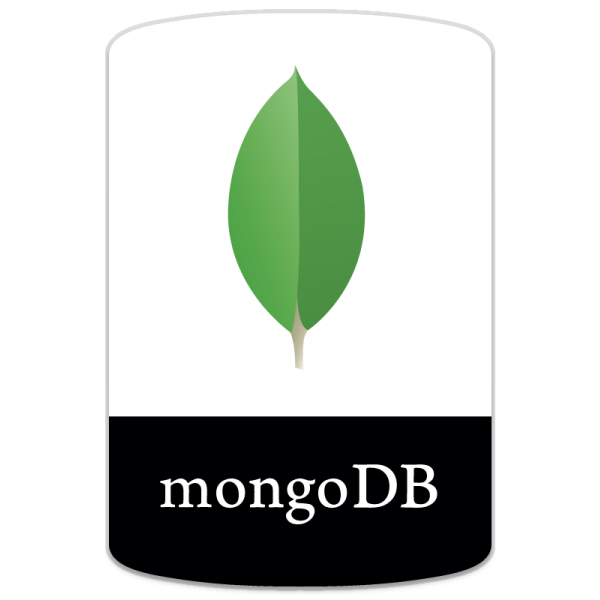
\includegraphics[width=40mm]{memoria/LaTeX/img/objetivos/mongo.png}
\end{figure}
    
    \item \textbf {Despliegue en la nube}: Hemos utilizado Amazon Web Service como plataforma de computación en la nube, lo que nos ha permitido un rápido despliegue de nuestra aplicación en producción. Consideramos que AWS además de ser pionero en este campo es una de las ofertas internacionales más importantes de la computación en la nube y compite directamente contra servicios como Microsoft Azure y Google Cloud Platform. 
    
        
\begin{figure}[H]
    \centering
    
\includegraphics[width=40mm]{memoria/LaTeX/img/objetivos/aws.png}
\end{figure}
 
\end{itemize}

\section{Metodología de trabajo}

Para la realización de todo el proyecto he seguido una metodología de trabajo que ha consistido en cinco diferentes fases:

\begin{itemize}

\item \textbf {Primera fase}: Es una fase de iniciación cuyo objetivo principal es el de aprender todo lo que tenga que ver con el desarrollo web. En esta fase deberíamos de dejar conceptos básicos aclarados y empezar a manejar alguna herramienta de control de versiones como Git. Es muy recomendable en esta primera fase empezar a manejar los lenguajes de programación que quieras utilizar en el futuro.

\item \textbf {Segunda fase}: Una vez que tenemos cierta destreza con el desarrollo, empezamos a enfocar nuestra aplicación decidiendo que tecnologías son las que mejor nos van a venir para nuestro modelo de aplicación. Esta fase es vital para la continuación del proyecto, ya que la mala elección de una tecnología nos puede llevar mucho tiempo.

\item \textbf {Tercera fase}: Una vez que tenemos claro que tecnologías vamos a utilizar en nuestra aplicación, comenzamos con una sencilla aplicación que utilice todas las tecnologías que estarán implicadas en nuestra aplicación. Esto nos servirá para tener una sencilla estructura de lo que queremos montar.

\item \textbf {Cuarta fase}: Cuando tengamos claros los conceptos, manejemos los lenguajes de programación necesarios y tengamos montado una sencilla aplicación con las tecnologías que hemos seleccionado para nuestro proyecto, es momento de empezar a dar forma a nuestras ideas. Esta fase es quizás la más emocionante de todas ya que empiezas a dar cuerpo a lo aprendido hasta ahora. 

\item \textbf {Quinta fase}: Cuando tengamos nuestra aplicación completamente desarrollada y haciendo lo que nosotros queremos, es el momento de subirla a alguna plataforma de computación en la nube. Esta ultima fase es quizás la mas sencilla y mas gratificante del proceso ya que es el momento de que tu trabajo sea contemplado por el resto del mundo.

\end{itemize}



